% Options for packages loaded elsewhere
\PassOptionsToPackage{unicode}{hyperref}
\PassOptionsToPackage{hyphens}{url}
\PassOptionsToPackage{dvipsnames,svgnames,x11names}{xcolor}
%
\documentclass[
  letterpaper,
  DIV=11,
  numbers=noendperiod]{scrreprt}

\usepackage{amsmath,amssymb}
\usepackage{iftex}
\ifPDFTeX
  \usepackage[T1]{fontenc}
  \usepackage[utf8]{inputenc}
  \usepackage{textcomp} % provide euro and other symbols
\else % if luatex or xetex
  \usepackage{unicode-math}
  \defaultfontfeatures{Scale=MatchLowercase}
  \defaultfontfeatures[\rmfamily]{Ligatures=TeX,Scale=1}
\fi
\usepackage{lmodern}
\ifPDFTeX\else  
    % xetex/luatex font selection
\fi
% Use upquote if available, for straight quotes in verbatim environments
\IfFileExists{upquote.sty}{\usepackage{upquote}}{}
\IfFileExists{microtype.sty}{% use microtype if available
  \usepackage[]{microtype}
  \UseMicrotypeSet[protrusion]{basicmath} % disable protrusion for tt fonts
}{}
\makeatletter
\@ifundefined{KOMAClassName}{% if non-KOMA class
  \IfFileExists{parskip.sty}{%
    \usepackage{parskip}
  }{% else
    \setlength{\parindent}{0pt}
    \setlength{\parskip}{6pt plus 2pt minus 1pt}}
}{% if KOMA class
  \KOMAoptions{parskip=half}}
\makeatother
\usepackage{xcolor}
\setlength{\emergencystretch}{3em} % prevent overfull lines
\setcounter{secnumdepth}{5}
% Make \paragraph and \subparagraph free-standing
\makeatletter
\ifx\paragraph\undefined\else
  \let\oldparagraph\paragraph
  \renewcommand{\paragraph}{
    \@ifstar
      \xxxParagraphStar
      \xxxParagraphNoStar
  }
  \newcommand{\xxxParagraphStar}[1]{\oldparagraph*{#1}\mbox{}}
  \newcommand{\xxxParagraphNoStar}[1]{\oldparagraph{#1}\mbox{}}
\fi
\ifx\subparagraph\undefined\else
  \let\oldsubparagraph\subparagraph
  \renewcommand{\subparagraph}{
    \@ifstar
      \xxxSubParagraphStar
      \xxxSubParagraphNoStar
  }
  \newcommand{\xxxSubParagraphStar}[1]{\oldsubparagraph*{#1}\mbox{}}
  \newcommand{\xxxSubParagraphNoStar}[1]{\oldsubparagraph{#1}\mbox{}}
\fi
\makeatother

\usepackage{color}
\usepackage{fancyvrb}
\newcommand{\VerbBar}{|}
\newcommand{\VERB}{\Verb[commandchars=\\\{\}]}
\DefineVerbatimEnvironment{Highlighting}{Verbatim}{commandchars=\\\{\}}
% Add ',fontsize=\small' for more characters per line
\usepackage{framed}
\definecolor{shadecolor}{RGB}{241,243,245}
\newenvironment{Shaded}{\begin{snugshade}}{\end{snugshade}}
\newcommand{\AlertTok}[1]{\textcolor[rgb]{0.68,0.00,0.00}{#1}}
\newcommand{\AnnotationTok}[1]{\textcolor[rgb]{0.37,0.37,0.37}{#1}}
\newcommand{\AttributeTok}[1]{\textcolor[rgb]{0.40,0.45,0.13}{#1}}
\newcommand{\BaseNTok}[1]{\textcolor[rgb]{0.68,0.00,0.00}{#1}}
\newcommand{\BuiltInTok}[1]{\textcolor[rgb]{0.00,0.23,0.31}{#1}}
\newcommand{\CharTok}[1]{\textcolor[rgb]{0.13,0.47,0.30}{#1}}
\newcommand{\CommentTok}[1]{\textcolor[rgb]{0.37,0.37,0.37}{#1}}
\newcommand{\CommentVarTok}[1]{\textcolor[rgb]{0.37,0.37,0.37}{\textit{#1}}}
\newcommand{\ConstantTok}[1]{\textcolor[rgb]{0.56,0.35,0.01}{#1}}
\newcommand{\ControlFlowTok}[1]{\textcolor[rgb]{0.00,0.23,0.31}{\textbf{#1}}}
\newcommand{\DataTypeTok}[1]{\textcolor[rgb]{0.68,0.00,0.00}{#1}}
\newcommand{\DecValTok}[1]{\textcolor[rgb]{0.68,0.00,0.00}{#1}}
\newcommand{\DocumentationTok}[1]{\textcolor[rgb]{0.37,0.37,0.37}{\textit{#1}}}
\newcommand{\ErrorTok}[1]{\textcolor[rgb]{0.68,0.00,0.00}{#1}}
\newcommand{\ExtensionTok}[1]{\textcolor[rgb]{0.00,0.23,0.31}{#1}}
\newcommand{\FloatTok}[1]{\textcolor[rgb]{0.68,0.00,0.00}{#1}}
\newcommand{\FunctionTok}[1]{\textcolor[rgb]{0.28,0.35,0.67}{#1}}
\newcommand{\ImportTok}[1]{\textcolor[rgb]{0.00,0.46,0.62}{#1}}
\newcommand{\InformationTok}[1]{\textcolor[rgb]{0.37,0.37,0.37}{#1}}
\newcommand{\KeywordTok}[1]{\textcolor[rgb]{0.00,0.23,0.31}{\textbf{#1}}}
\newcommand{\NormalTok}[1]{\textcolor[rgb]{0.00,0.23,0.31}{#1}}
\newcommand{\OperatorTok}[1]{\textcolor[rgb]{0.37,0.37,0.37}{#1}}
\newcommand{\OtherTok}[1]{\textcolor[rgb]{0.00,0.23,0.31}{#1}}
\newcommand{\PreprocessorTok}[1]{\textcolor[rgb]{0.68,0.00,0.00}{#1}}
\newcommand{\RegionMarkerTok}[1]{\textcolor[rgb]{0.00,0.23,0.31}{#1}}
\newcommand{\SpecialCharTok}[1]{\textcolor[rgb]{0.37,0.37,0.37}{#1}}
\newcommand{\SpecialStringTok}[1]{\textcolor[rgb]{0.13,0.47,0.30}{#1}}
\newcommand{\StringTok}[1]{\textcolor[rgb]{0.13,0.47,0.30}{#1}}
\newcommand{\VariableTok}[1]{\textcolor[rgb]{0.07,0.07,0.07}{#1}}
\newcommand{\VerbatimStringTok}[1]{\textcolor[rgb]{0.13,0.47,0.30}{#1}}
\newcommand{\WarningTok}[1]{\textcolor[rgb]{0.37,0.37,0.37}{\textit{#1}}}

\providecommand{\tightlist}{%
  \setlength{\itemsep}{0pt}\setlength{\parskip}{0pt}}\usepackage{longtable,booktabs,array}
\usepackage{calc} % for calculating minipage widths
% Correct order of tables after \paragraph or \subparagraph
\usepackage{etoolbox}
\makeatletter
\patchcmd\longtable{\par}{\if@noskipsec\mbox{}\fi\par}{}{}
\makeatother
% Allow footnotes in longtable head/foot
\IfFileExists{footnotehyper.sty}{\usepackage{footnotehyper}}{\usepackage{footnote}}
\makesavenoteenv{longtable}
\usepackage{graphicx}
\makeatletter
\def\maxwidth{\ifdim\Gin@nat@width>\linewidth\linewidth\else\Gin@nat@width\fi}
\def\maxheight{\ifdim\Gin@nat@height>\textheight\textheight\else\Gin@nat@height\fi}
\makeatother
% Scale images if necessary, so that they will not overflow the page
% margins by default, and it is still possible to overwrite the defaults
% using explicit options in \includegraphics[width, height, ...]{}
\setkeys{Gin}{width=\maxwidth,height=\maxheight,keepaspectratio}
% Set default figure placement to htbp
\makeatletter
\def\fps@figure{htbp}
\makeatother
% definitions for citeproc citations
\NewDocumentCommand\citeproctext{}{}
\NewDocumentCommand\citeproc{mm}{%
  \begingroup\def\citeproctext{#2}\cite{#1}\endgroup}
\makeatletter
 % allow citations to break across lines
 \let\@cite@ofmt\@firstofone
 % avoid brackets around text for \cite:
 \def\@biblabel#1{}
 \def\@cite#1#2{{#1\if@tempswa , #2\fi}}
\makeatother
\newlength{\cslhangindent}
\setlength{\cslhangindent}{1.5em}
\newlength{\csllabelwidth}
\setlength{\csllabelwidth}{3em}
\newenvironment{CSLReferences}[2] % #1 hanging-indent, #2 entry-spacing
 {\begin{list}{}{%
  \setlength{\itemindent}{0pt}
  \setlength{\leftmargin}{0pt}
  \setlength{\parsep}{0pt}
  % turn on hanging indent if param 1 is 1
  \ifodd #1
   \setlength{\leftmargin}{\cslhangindent}
   \setlength{\itemindent}{-1\cslhangindent}
  \fi
  % set entry spacing
  \setlength{\itemsep}{#2\baselineskip}}}
 {\end{list}}
\usepackage{calc}
\newcommand{\CSLBlock}[1]{\hfill\break\parbox[t]{\linewidth}{\strut\ignorespaces#1\strut}}
\newcommand{\CSLLeftMargin}[1]{\parbox[t]{\csllabelwidth}{\strut#1\strut}}
\newcommand{\CSLRightInline}[1]{\parbox[t]{\linewidth - \csllabelwidth}{\strut#1\strut}}
\newcommand{\CSLIndent}[1]{\hspace{\cslhangindent}#1}

\KOMAoption{captions}{tableheading}
\makeatletter
\@ifpackageloaded{tcolorbox}{}{\usepackage[skins,breakable]{tcolorbox}}
\@ifpackageloaded{fontawesome5}{}{\usepackage{fontawesome5}}
\definecolor{quarto-callout-color}{HTML}{909090}
\definecolor{quarto-callout-note-color}{HTML}{0758E5}
\definecolor{quarto-callout-important-color}{HTML}{CC1914}
\definecolor{quarto-callout-warning-color}{HTML}{EB9113}
\definecolor{quarto-callout-tip-color}{HTML}{00A047}
\definecolor{quarto-callout-caution-color}{HTML}{FC5300}
\definecolor{quarto-callout-color-frame}{HTML}{acacac}
\definecolor{quarto-callout-note-color-frame}{HTML}{4582ec}
\definecolor{quarto-callout-important-color-frame}{HTML}{d9534f}
\definecolor{quarto-callout-warning-color-frame}{HTML}{f0ad4e}
\definecolor{quarto-callout-tip-color-frame}{HTML}{02b875}
\definecolor{quarto-callout-caution-color-frame}{HTML}{fd7e14}
\makeatother
\makeatletter
\@ifpackageloaded{bookmark}{}{\usepackage{bookmark}}
\makeatother
\makeatletter
\@ifpackageloaded{caption}{}{\usepackage{caption}}
\AtBeginDocument{%
\ifdefined\contentsname
  \renewcommand*\contentsname{Indice}
\else
  \newcommand\contentsname{Indice}
\fi
\ifdefined\listfigurename
  \renewcommand*\listfigurename{Elenco delle Figure}
\else
  \newcommand\listfigurename{Elenco delle Figure}
\fi
\ifdefined\listtablename
  \renewcommand*\listtablename{Elenco delle Tabelle}
\else
  \newcommand\listtablename{Elenco delle Tabelle}
\fi
\ifdefined\figurename
  \renewcommand*\figurename{Figura}
\else
  \newcommand\figurename{Figura}
\fi
\ifdefined\tablename
  \renewcommand*\tablename{Tabella}
\else
  \newcommand\tablename{Tabella}
\fi
}
\@ifpackageloaded{float}{}{\usepackage{float}}
\floatstyle{ruled}
\@ifundefined{c@chapter}{\newfloat{codelisting}{h}{lop}}{\newfloat{codelisting}{h}{lop}[chapter]}
\floatname{codelisting}{Lista}
\newcommand*\listoflistings{\listof{codelisting}{Elenco degli Elenchi}}
\usepackage{amsthm}
\theoremstyle{definition}
\newtheorem{example}{Esempio}[chapter]
\theoremstyle{remark}
\AtBeginDocument{\renewcommand*{\proofname}{Dimostrazione}}
\newtheorem*{remark}{Osservazione}
\newtheorem*{solution}{Soluzione}
\newtheorem{refremark}{Osservazione}[chapter]
\newtheorem{refsolution}{Soluzione}[chapter]
\makeatother
\makeatletter
\makeatother
\makeatletter
\@ifpackageloaded{caption}{}{\usepackage{caption}}
\@ifpackageloaded{subcaption}{}{\usepackage{subcaption}}
\makeatother

\ifLuaTeX
\usepackage[bidi=basic]{babel}
\else
\usepackage[bidi=default]{babel}
\fi
\babelprovide[main,import]{italian}
% get rid of language-specific shorthands (see #6817):
\let\LanguageShortHands\languageshorthands
\def\languageshorthands#1{}
\ifLuaTeX
  \usepackage{selnolig}  % disable illegal ligatures
\fi
\usepackage{bookmark}

\IfFileExists{xurl.sty}{\usepackage{xurl}}{} % add URL line breaks if available
\urlstyle{same} % disable monospaced font for URLs
\hypersetup{
  pdftitle={Psicometria},
  pdfauthor={Corrado Caudek},
  pdflang={it},
  colorlinks=true,
  linkcolor={blue},
  filecolor={Maroon},
  citecolor={Blue},
  urlcolor={Blue},
  pdfcreator={LaTeX via pandoc}}


\title{Psicometria}
\usepackage{etoolbox}
\makeatletter
\providecommand{\subtitle}[1]{% add subtitle to \maketitle
  \apptocmd{\@title}{\par {\large #1 \par}}{}{}
}
\makeatother
\subtitle{Anno Accademico 2024/2025}
\author{Corrado Caudek}
\date{2024-11-27}

\begin{document}
\maketitle

\renewcommand*\contentsname{Indice}
{
\hypersetup{linkcolor=}
\setcounter{tocdepth}{4}
\tableofcontents
}

\bookmarksetup{startatroot}

\chapter*{Benvenuti}\label{benvenuti}
\addcontentsline{toc}{chapter}{Benvenuti}

\markboth{Benvenuti}{Benvenuti}

Benvenuti nel sito web dell'insegnamento di
\href{https://www.unifi.it/index.php?module=ofform2&mode=1&cmd=3&AA=2023&afId=689762}{Psicometria},
parte del
\href{https://www.psicologia.unifi.it/vp-130-scienze-e-tecniche-psicologiche-l-24.html}{Corso
di Laurea in Scienze e Tecniche Psicologiche}
dell'\href{https://www.unifi.it/}{Università degli Studi di Firenze}.

\section*{Descrizione}\label{descrizione}
\addcontentsline{toc}{section}{Descrizione}

\markright{Descrizione}

L'insegnamento offre una formazione teorico-pratica nell'ambito
dell'inferenza statistica, con un focus particolare sulle applicazioni
in campo psicologico. Attraverso esercitazioni pratiche in Python e R,
gli studenti acquisiranno competenze nell'analisi di dati e nell'uso di
modelli statistici avanzati.

\begin{itemize}
\tightlist
\item
  \textbf{Anno Accademico}: 2024-2025
\item
  \textbf{Codice Insegnamento}: B000286
\item
  \textbf{Orario e Luogo}: Lunedì e Martedì (8:30-10:30), Giovedì
  (11:30-13:30), Plesso didattico La Torretta.
\end{itemize}

\begin{tcolorbox}[enhanced jigsaw, leftrule=.75mm, title=\textcolor{quarto-callout-note-color}{\faInfo}\hspace{0.5em}{Nota}, colframe=quarto-callout-note-color-frame, colbacktitle=quarto-callout-note-color!10!white, arc=.35mm, toptitle=1mm, breakable, rightrule=.15mm, opacityback=0, bottomrule=.15mm, toprule=.15mm, bottomtitle=1mm, coltitle=black, titlerule=0mm, left=2mm, opacitybacktitle=0.6, colback=white]

Questo sito web è la fonte ufficiale per il programma
dell'insegnamento~\emph{B000286 - Psicometria}~e le modalità d'esame.

\end{tcolorbox}

\section*{Struttura dell'Insegnamento}\label{struttura-dellinsegnamento}
\addcontentsline{toc}{section}{Struttura dell'Insegnamento}

\markright{Struttura dell'Insegnamento}

L'insegnamento è organizzato in diverse sezioni, ciascuna dedicata a uno
specifico argomento chiave.

\begin{enumerate}
\def\labelenumi{\arabic{enumi}.}
\tightlist
\item
  \textbf{Fondamenti}: Introduzione ai concetti statistici di base.
\item
  \textbf{Inferenza Bayesiana}: Applicazioni avanzate dell'inferenza
  causale.
\item
  \textbf{Programmazione in Python e R}: Utilizzo pratico per l'analisi
  dati.
\item
  \textbf{Visualizzazione dei Dati}: Tecniche per interpretare e
  comunicare risultati.
\end{enumerate}

\href{syllabus/syllabus.pdf}{Consulta il syllabus completo} per
ulteriori dettagli.

\section*{Materiale Didattico}\label{materiale-didattico}
\addcontentsline{toc}{section}{Materiale Didattico}

\markright{Materiale Didattico}

Il presente sito web ospita la \textbf{dispensa ufficiale del corso},
contenente tutte le note e i materiali relativi alle lezioni. Per quanto
riguarda le esercitazioni pratiche e gli esempi applicativi, è possibile
accedere al sito dedicato, disponibile al seguente indirizzo:
\href{https://ccaudek.github.io/psicometria-esercizi/}{Psicometria
Esercizi}. Entrambi i materiali sono forniti gratuitamente agli
studenti, senza necessità di ulteriori acquisti.

\bookmarksetup{startatroot}

\chapter*{Prefazione}\label{prefazione}
\addcontentsline{toc}{chapter}{Prefazione}

\markboth{Prefazione}{Prefazione}

Come possiamo migliorare l'analisi dei dati psicologici per renderla più
affidabile e robusta? È possibile affrontare questa sfida semplicemente
applicando una serie di algoritmi o procedure standard? L'analisi dei
dati in psicologia può davvero essere ridotta a un insieme di
``ricette'' preconfezionate
(\citeproc{ref-McElreath_rethinking}{McElreath, 2020})?

Queste domande ci portano a riflettere sulla natura stessa dell'analisi
dei dati psicologici. A differenza di ciò che suggerisce l'approccio
frequentista del test dell'ipotesi nulla, l'analisi dei dati non è una
disciplina che si esaurisce con l'applicazione meccanica di metodi
predefiniti. Anzi, considerare l'analisi dei dati come un insieme di
procedure automatiche contribuisce a uno dei problemi più gravi della
psicologia contemporanea: la crisi della replicabilità dei risultati
(\citeproc{ref-korbmacher2023replication}{Korbmacher et al., 2023}).

Ma perché la replicabilità è così cruciale? Se i risultati delle
ricerche psicologiche non sono replicabili, significa che la nostra
comprensione dei fenomeni psicologici è superficiale e inaffidabile.
Questo non è solo un problema teorico o accademico; ha implicazioni
dirette sulle applicazioni pratiche della psicologia. Se le basi
scientifiche sono incerte, anche le strategie di intervento psicologico
rischiano di essere inefficaci o addirittura dannose
(\citeproc{ref-funder2014improving}{Funder et al., 2014};
\citeproc{ref-ioannidis2019have}{Ioannidis, 2019};
\citeproc{ref-shrout2018psychology}{Shrout \& Rodgers, 2018};
\citeproc{ref-tackett2019psychology}{Tackett et al., 2019}).

Perché le pratiche di analisi dei dati derivanti dal frequentismo
potrebbero contribuire a questa crisi? In che modo gli incentivi
accademici influenzano la qualità della ricerca psicologica? E,
soprattutto, quali alternative abbiamo per migliorare l'affidabilità e
la validità delle nostre conclusioni?

L'analisi bayesiana emerge come una delle proposte per superare i limiti
dell'approccio frequentista (\citeproc{ref-gelman1995bayesian}{Gelman et
al., 1995}). Tuttavia, è sufficiente abbandonare l'inferenza
frequentista per risolvere i problemi della psicologia? Come possiamo
integrare metodi robusti e flessibili, come quelli bayesiani, con una
comprensione più approfondita e trasparente dei fenomeni psicologici?

In questo corso, esploreremo queste domande, cercando di identificare le
``buone pratiche'' dell'analisi dei dati psicologici. Discuteremo i
limiti delle metodologie attuali, esamineremo le cause sottostanti della
crisi della replicabilità e valuteremo come l'adozione di metodi
avanzati, come l'inferenza bayesiana e la modellazione causale, possa
offrire soluzioni efficaci
(\citeproc{ref-oberauer2019addressing}{Oberauer \& Lewandowsky, 2019};
\citeproc{ref-wagenmakers2018bayesian}{Wagenmakers et al., 2018};
\citeproc{ref-yarkoni2022generalizability}{Yarkoni, 2022}). Il nostro
obiettivo è fornire una visione critica e costruttiva, che non solo
identifichi le sfide della ricerca psicologica, ma proponga anche
percorsi concreti per migliorare la qualità e l'affidabilità della
scienza psicologica.

\part{Programmazione}

\chapter{Calendario delle lezioni}\label{calendario-delle-lezioni}

Il calendario didattico prevede 32 incontri, con un esame parziale a
metà corso e gli ultimi tre incontri riservati a un secondo esame
parziale e alle presentazioni degli studenti.

\begin{longtable}[]{@{}
  >{\raggedright\arraybackslash}p{(\columnwidth - 6\tabcolsep) * \real{0.1757}}
  >{\raggedright\arraybackslash}p{(\columnwidth - 6\tabcolsep) * \real{0.1757}}
  >{\raggedright\arraybackslash}p{(\columnwidth - 6\tabcolsep) * \real{0.4730}}
  >{\raggedright\arraybackslash}p{(\columnwidth - 6\tabcolsep) * \real{0.1757}}@{}}
\toprule\noalign{}
\begin{minipage}[b]{\linewidth}\raggedright
\textbf{Incontro}
\end{minipage} & \begin{minipage}[b]{\linewidth}\raggedright
\textbf{Data}
\end{minipage} & \begin{minipage}[b]{\linewidth}\raggedright
\textbf{Argomento}
\end{minipage} & \begin{minipage}[b]{\linewidth}\raggedright
\textbf{Orario}
\end{minipage} \\
\midrule\noalign{}
\endhead
\bottomrule\noalign{}
\endlastfoot
1 & 3 marzo & Presentazione del corso, struttura e obiettivi &
8:30-10:30 \\
2 & 4 marzo & Introduzione a Python e R per l'analisi dei dati &
8:30-10:30 \\
3 & 6 marzo & Exploratory Data Analysis & 11:30-13:30 \\
4 & 10 marzo & Fondamenti di probabilità & 8:30-10:30 \\
5 & 11 marzo & Spazi di probabilità e variabili casuali & 8:30-10:30 \\
6 & 13 marzo & Distribuzioni di probabilità discreta & 11:30-13:30 \\
7 & 17 marzo & Distribuzioni di probabilità continua & 8:30-10:30 \\
8 & 18 marzo & Teorema di Bayes e inferenza Bayesiana & 8:30-10:30 \\
9 & 20 marzo & Priori coniugati e metodo basato su griglia &
11:30-13:30 \\
10 & 24 marzo & Metodi Monte Carlo e algoritmi MCMC & 8:30-10:30 \\
11 & 25 marzo & Introduzione a Stan e programmazione probabilistica &
8:30-10:30 \\
12 & 27 marzo & Predizione bayesiana & 11:30-13:30 \\
13 & 31 marzo & Sintesi e diagnostica della distribuzione a posteriori &
8:30-10:30 \\
14 & 1 aprile & Modello gaussiano, poisson, esponenziale, a mistura &
8:30-10:30 \\
15 & 3 aprile & Modello categoriale e gerarchico & 11:30-13:30 \\
16 & 7 aprile & Modello lineare bivariato, OLS & 8:30-10:30 \\
17 & 8 aprile & Elementi di algebra lineare e regressione multipla &
8:30-10:30 \\
18 & 10 aprile & Analisi della covarianza, interazioni statistiche &
11:30-13:30 \\
\end{longtable}

\textbf{Pausa di Pasqua}

\begin{longtable}[]{@{}
  >{\raggedright\arraybackslash}p{(\columnwidth - 6\tabcolsep) * \real{0.1781}}
  >{\raggedright\arraybackslash}p{(\columnwidth - 6\tabcolsep) * \real{0.1781}}
  >{\raggedright\arraybackslash}p{(\columnwidth - 6\tabcolsep) * \real{0.4658}}
  >{\raggedright\arraybackslash}p{(\columnwidth - 6\tabcolsep) * \real{0.1781}}@{}}
\toprule\noalign{}
\begin{minipage}[b]{\linewidth}\raggedright
\textbf{Incontro}
\end{minipage} & \begin{minipage}[b]{\linewidth}\raggedright
\textbf{Data}
\end{minipage} & \begin{minipage}[b]{\linewidth}\raggedright
\textbf{Argomento}
\end{minipage} & \begin{minipage}[b]{\linewidth}\raggedright
\textbf{Orario}
\end{minipage} \\
\midrule\noalign{}
\endhead
\bottomrule\noalign{}
\endlastfoot
19 & 15 aprile & Esame parziale & 8:30-10:30 \\
20 & 17 aprile & Modello lineare gerarchico e modelli lineari misti &
11:30-13:30 \\
21 & 22 aprile & Inferenza causale: concetti di base & 8:30-10:30 \\
22 & 24 aprile & GLM, regressione logistica e binomiale & 11:30-13:30 \\
23 & 28 aprile & Entropia e teoria dell'informazione & 8:30-10:30 \\
24 & 29 aprile & Comparazione di modelli con entropia & 8:30-10:30 \\
25 & 6 maggio & Analisi dei dati longitudinali e modelli dinamici &
8:30-10:30 \\
26 & 8 maggio & Modelli cognitivi & 11:30-13:30 \\
27 & 12 maggio & Test di ipotesi frequentista & 8:30-10:30 \\
28 & 13 maggio & Intervalli di confidenza frequentisti & 8:30-10:30 \\
29 & 15 maggio & Crisi della replicazione & 11:30-13:30 \\
\end{longtable}

\textbf{Esame parziale e presentazioni finali}

\begin{longtable}[]{@{}llll@{}}
\toprule\noalign{}
\textbf{Incontro} & \textbf{Data} & \textbf{Argomento} &
\textbf{Orario} \\
\midrule\noalign{}
\endhead
\bottomrule\noalign{}
\endlastfoot
30 & 19 maggio & Esame parziale finale & 8:30-10:30 \\
31 & 20 maggio & Presentazioni dei progetti & 8:30-10:30 \\
32 & 22 maggio & Presentazioni dei progetti & 11:30-13:30 \\
\end{longtable}

\begin{center}\rule{0.5\linewidth}{0.5pt}\end{center}

\section{Calendario delle relazioni in
itinere}\label{calendario-delle-relazioni-in-itinere}

Le relazioni di avanzamento del progetto di gruppo dovranno essere
consegnate entro le scadenze stabilite. Ogni gruppo dovrà presentare un
unico elaborato.

\begin{longtable}[]{@{}
  >{\raggedright\arraybackslash}p{(\columnwidth - 2\tabcolsep) * \real{0.2500}}
  >{\raggedright\arraybackslash}p{(\columnwidth - 2\tabcolsep) * \real{0.7500}}@{}}
\toprule\noalign{}
\begin{minipage}[b]{\linewidth}\raggedright
\textbf{Data di Scadenza}
\end{minipage} & \begin{minipage}[b]{\linewidth}\raggedright
\textbf{Contenuto della Relazione}
\end{minipage} \\
\midrule\noalign{}
\endhead
\bottomrule\noalign{}
\endlastfoot
18 marzo & \textbf{Relazione 1:} Importazione dei dati, data wrangling,
data tidying, dizionario dei dati, statistiche descrittive \\
25 marzo & \textbf{Relazione 2:} Priori coniugati e metodo basato su
griglia \\
31 marzo & \textbf{Relazione 3:} Metodi Monte Carlo e algoritmi MCMC \\
7 aprile & \textbf{Relazione 4:} Regressione lineare \\
8 maggio & \textbf{Relazione 5:} Confronto di modelli \\
18 maggio & \textbf{Relazione 6:} Analisi frequentista; limiti
dell'approccio frequentista \\
\end{longtable}

Ogni relazione rappresenta una tappa del progetto di gruppo, che
culminerà nella presentazione finale durante gli ultimi incontri del
corso.

\part{Fondamenti}

\chapter*{Introduzione}\label{introduzione}
\addcontentsline{toc}{chapter}{Introduzione}

\markboth{Introduzione}{Introduzione}

La data science è un campo che si sviluppa all'intersezione tra la
statistica e l'informatica. La statistica fornisce una serie di
metodologie per analizzare i dati e ottenere informazioni significative,
mentre l'informatica si occupa dello sviluppo di software e strumenti
per implementare tali metodologie. In questa sezione della dispensa,
approfondiremo alcuni concetti fondamentali della statistica e della
misurazione psicologica. Considereremo anche in termini generali quali
sono gli obiettivi e i limiti dell'analisi dei dati psicologici.

\chapter{Abbracciare l'incertezza}\label{sec-uncertainty}

\textbf{Prerequisiti}

\textbf{Concetti e competenze chiave}

\section{Introduzione}\label{introduzione-1}

L'espressione ``abbracciare l'incertezza'' è tra le più emblematiche nel
panorama della statistica bayesiana. In questo capitolo, approfondiremo
il significato di questa affermazione, seguendo la trattazione
introduttiva proposta nel primo capitolo di \emph{Understanding
Uncertainty} di Lindley
(\citeproc{ref-lindley2013understanding}{Lindley, 2013}).

\section{L'incertezza nella ricerca
psicologica}\label{lincertezza-nella-ricerca-psicologica}

L'incertezza rappresenta un elemento cruciale non solo nella statistica,
ma in tutte le discipline scientifiche, con particolare rilievo per la
psicologia, che affronta fenomeni complessi e difficili da misurare.
Nell'indagare processi cognitivi, emozioni e comportamenti, i
ricercatori si confrontano con dati complessi, spesso ambigui e
suscettibili di interpretazioni molteplici. Sebbene alcune affermazioni
possano essere sostenute con elevata confidenza o confutate con
certezza, la maggior parte delle ipotesi scientifiche si colloca in una
zona grigia dominata dall'incertezza.

L'obiettivo di questo insegnamento è guidare gli studenti nella
comprensione e nella gestione dell'incertezza nella ricerca psicologica,
adottando l'approccio bayesiano all'analisi dei dati. Questo metodo,
basato sulla quantificazione e sull'aggiornamento delle credenze alla
luce di nuove evidenze, fornirà agli studenti gli strumenti per
affrontare l'incertezza in modo rigoroso e sistematico, sia nella
carriera accademica sia nella pratica clinica.

\section{La natura soggettiva
dell'incertezza}\label{la-natura-soggettiva-dellincertezza}

Un elemento cruciale dell'incertezza, spesso trascurato, è la sua
dimensione soggettiva. De Finetti
(\citeproc{ref-definetti1970teoria}{Finetti, 1970}) ha evidenziato come
l'incertezza sia, almeno in parte, una questione personale: ciò che è
incerto per uno psicologo può non esserlo per un altro, in funzione
delle loro esperienze, conoscenze pregresse e interpretazioni dei dati
disponibili. Anche di fronte a una stessa questione, due ricercatori
possono condividere un'incertezza comune, ma con gradi di intensità
diversi.

Questa componente soggettiva è particolarmente significativa in
psicologia, dove le differenze individuali e culturali influenzano la
percezione e l'interpretazione dei fenomeni. L'approccio bayesiano offre
un potente strumento per affrontare questa soggettività, consentendo di
quantificare le differenze tra credenze individuali e di aggiornarle in
modo coerente sulla base di nuove evidenze oggettive.

\section{L'onnipresenza
dell'incertezza}\label{lonnipresenza-dellincertezza}

L'incertezza pervade ogni aspetto della ricerca psicologica. Ogni
esperimento, misurazione o interpretazione dei dati comporta un margine
di incertezza. Questa condizione è particolarmente evidente nello studio
di fenomeni complessi come il comportamento umano o i processi mentali,
dove innumerevoli variabili interagiscono, molte delle quali difficili
da misurare o controllare con precisione.

Tuttavia, l'incertezza non deve essere vista come un ostacolo
insormontabile. Al contrario, riconoscerla e quantificarla può favorire
una comprensione più profonda e realistica dei fenomeni psicologici.
Attraverso l'approccio bayesiano, diventa possibile integrare
l'incertezza nel processo di indagine scientifica, trattandola non come
un limite, ma come una risorsa.

\section{Superare la soppressione
dell'incertezza}\label{superare-la-soppressione-dellincertezza}

Nonostante la sua onnipresenza, l'incertezza è spesso ignorata o
minimizzata nella comunicazione scientifica. Questo può avvenire
attraverso interpretazioni eccessivamente ottimistiche dei risultati, la
presentazione di conclusioni come fatti certi, o una riluttanza a
riconoscere i limiti degli studi condotti. Tale atteggiamento, sebbene
comprensibile, può condurre a conclusioni errate e a una visione
distorta della realtà.

L'approccio bayesiano permette di affrontare l'incertezza in modo
esplicito e costruttivo. Fornendo un quadro rigoroso per quantificarla,
analizzarla e comunicarla chiaramente, migliora la trasparenza della
ricerca e promuove conclusioni più oneste e accurate.

\section{I benefici dell'incertezza}\label{i-benefici-dellincertezza}

Contrariamente a quanto si possa pensare, l'incertezza offre numerosi
vantaggi per la ricerca psicologica:

\begin{itemize}
\tightlist
\item
  \textbf{Stimola l'esplorazione scientifica}: La consapevolezza
  dell'incertezza incoraggia i ricercatori a formulare nuove ipotesi e a
  migliorare i metodi di studio.
\item
  \textbf{Promuove l'onestà intellettuale}: Accettare l'incertezza rende
  i ricercatori più cauti e aperti a prospettive alternative.
\item
  \textbf{Migliora la qualità delle analisi}: Integrare l'incertezza
  porta a disegni sperimentali più robusti e interpretazioni più
  accurate.
\item
  \textbf{Facilita la collaborazione interdisciplinare}: Riconoscere i
  limiti delle proprie conoscenze stimola la ricerca di input da altri
  esperti.
\item
  \textbf{Riflette la complessità dei fenomeni psicologici}:
  L'incertezza è intrinseca ai processi mentali e riconoscerla consente
  di rappresentarli in modo più realistico.
\end{itemize}

\section{Tipi di incertezza}\label{tipi-di-incertezza}

L'incertezza nella ricerca può essere classificata in tre categorie
principali, in base alla sua origine: aleatoria, epistemica e ontologica
(\citeproc{ref-gansch2020system}{Gansch \& Adee, 2020}).

\subsection{Incertezza Aleatoria}\label{incertezza-aleatoria}

L'incertezza aleatoria è intrinseca alla natura casuale di un processo e
non può essere eliminata per un dato modello probabilistico. Essa è
considerata irreducibile e viene quantificata tramite distribuzioni
probabilistiche. Ad esempio, nella misurazione della risposta di un
individuo a uno stimolo, la variabilità intrinseca nel comportamento
umano, dovuta a fattori imprevedibili, rappresenta un caso di incertezza
aleatoria. Questo tipo di incertezza è una caratteristica fondamentale
di molti fenomeni psicologici e biologici.

\subsection{Incertezza Epistemica}\label{incertezza-epistemica}

L'incertezza epistemica deriva dalla conoscenza limitata o incompleta di
un fenomeno. Essa rappresenta il ``noto-ignoto'', cioè ciò che sappiamo
di non sapere, ed è legata alle semplificazioni insite in ogni modello
scientifico. Ad esempio, un modello psicologico che non consideri le
influenze culturali o ambientali potrebbe risultare incompleto,
introducendo incertezza epistemica. Diversamente dall'incertezza
aleatoria, l'incertezza epistemica può essere ridotta attraverso il
miglioramento dei modelli, l'inclusione di variabili rilevanti o la
raccolta di ulteriori dati.

\subsection{Incertezza Ontologica}\label{incertezza-ontologica}

L'incertezza ontologica riguarda l'\,``ignoto-ignoto'', ovvero aspetti
di un sistema che non sono ancora stati identificati. In psicologia,
questo potrebbe riferirsi a variabili o processi non ancora scoperti che
influenzano un comportamento. Ad esempio, studiando i disturbi mentali,
potrebbero emergere nuovi fattori di rischio precedentemente
sconosciuti.

\section{Il calcolo dell'incertezza nell'approccio
bayesiano}\label{il-calcolo-dellincertezza-nellapproccio-bayesiano}

L'insegnamento si propone di fornire agli studenti strumenti per
affrontare e quantificare l'incertezza attraverso l'approccio bayesiano
(\citeproc{ref-gelman1995bayesian}{Gelman et al., 1995}). Fondato sul
teorema di Bayes, questo metodo rappresenta un quadro teorico rigoroso e
sistematico per aggiornare le credenze alla luce di nuove evidenze,
configurandosi come una componente centrale della metodologia
scientifica.

Il processo si basa su quattro passaggi essenziali. In primo luogo, si
parte dalla quantificazione delle credenze iniziali, note come
\emph{prior}, che rappresentano le conoscenze pregresse o le ipotesi
relative a un determinato fenomeno psicologico. Successivamente, si
analizza la forza delle evidenze empiriche fornite dai dati raccolti,
formalizzata nella \emph{likelihood}. Queste due informazioni vengono
combinate per generare le credenze aggiornate, chiamate
\emph{posterior}, che sintetizzano la conoscenza disponibile integrando
i dati empirici e le ipotesi iniziali. Infine, le credenze aggiornate
possono essere utilizzate per prendere decisioni più informate,
pianificare ricerche future e orientare interventi.

\subsection{Il ruolo delle credenze e delle decisioni nella ricerca
psicologica}\label{il-ruolo-delle-credenze-e-delle-decisioni-nella-ricerca-psicologica}

Le credenze rivestono un ruolo fondamentale nella ricerca psicologica,
influenzando tutte le fasi del processo scientifico, dalla progettazione
degli esperimenti all'interpretazione dei risultati, fino alla scelta di
interventi clinici. L'approccio bayesiano si distingue per la sua
capacità di esplicitare e formalizzare queste credenze, consentendo di
aggiornare il loro contenuto in modo coerente e trasparente man mano che
emergono nuove evidenze.

Questo metodo permette non solo di ottimizzare le decisioni basandosi su
informazioni aggiornate, ma anche di comunicare chiaramente l'incertezza
associata alle conclusioni, evidenziandone i limiti e garantendo
maggiore trasparenza scientifica. Affrontare l'incertezza come una
componente intrinseca della ricerca non solo migliora la qualità
dell'analisi, ma consente anche di promuovere un approccio più
realistico e rigoroso nello studio dei fenomeni psicologici.

In sintesi, l'approccio bayesiano offre un modello operativo per
integrare l'incertezza nel processo decisionale, trattandola non come un
ostacolo, ma come un elemento essenziale per una comprensione più
sfumata e accurata della realtà.

\section{Riflessioni Conclusive}\label{riflessioni-conclusive}

Questo insegnamento fornisce gli strumenti per applicare l'analisi
bayesiana nell'ambito dei dati psicologici, insegnando a considerare
l'incertezza come una parte integrante e preziosa del processo
scientifico. Attraverso questo approccio, gli studenti potranno
acquisire una comprensione più raffinata e strutturata dei fenomeni
psicologici, integrando l'incertezza come elemento fondamentale per
interpretare i dati e formulare inferenze rigorose.

\section*{Bibliografia}\label{bibliografia}
\addcontentsline{toc}{section}{Bibliografia}

\markright{Bibliografia}

\chapter{Concetti chiave}\label{sec-key-notions}

\textbf{Prerequisiti}

\begin{itemize}
\tightlist
\item
  Leggere \href{../../figures/horoscopes.pdf}{Horoscopes}. L'ultimo
  capitolo di McElreath (\citeproc{ref-McElreath_rethinking}{2020})
  discute il contesto scientifico e culturale della statistica.
\item
  Leggere \href{https://theeffectbook.net}{The Effect: An Introduction
  to Research Design and Causality}. Focalizzati sul capitolo 10
  \emph{Treatment Effects}.
\end{itemize}

\textbf{Concetti e competenze chiave}

\begin{itemize}
\tightlist
\item
  Definizione di popolazione e campione.
\item
  Distinzione tra variabili indipendenti e dipendenti.
\item
  La matrice dei dati.
\item
  L'effetto delle variabili all'interno dell'analisi statistica.
\item
  I concetti di stima e inferenza.
\item
  Il concetto di modello psicologico.
\end{itemize}

\textbf{Preparazione del Notebook}

\section*{Introduzione}\label{introduzione-2}
\addcontentsline{toc}{section}{Introduzione}

\markright{Introduzione}

\begin{quote}
Most of the fundamental ideas of science are essentially simple, and
may, as a rule, be expressed in a language comprehensible to everyone.\\
(Einstein A and Infeld L, 1938)
\end{quote}

Questo capitolo introduce il contesto e i principi base dell'analisi dei
dati, con un focus su come le tecniche statistiche, combinate con una
solida teoria dei fenomeni, siano strumentali all'avanzamento delle
conoscenze scientifiche.

\begin{tcolorbox}[enhanced jigsaw, leftrule=.75mm, title=\textcolor{quarto-callout-note-color}{\faInfo}\hspace{0.5em}{Statistica}, colframe=quarto-callout-note-color-frame, colbacktitle=quarto-callout-note-color!10!white, arc=.35mm, toptitle=1mm, breakable, rightrule=.15mm, opacityback=0, bottomrule=.15mm, toprule=.15mm, bottomtitle=1mm, coltitle=black, titlerule=0mm, left=2mm, opacitybacktitle=0.6, colback=white]

Il termine ``statistica'' può assumere diversi significati, a seconda
del contesto in cui viene utilizzato.

\begin{itemize}
\tightlist
\item
  Nel primo senso, la statistica è una scienza e una disciplina che si
  occupa dello studio e dell'applicazione di metodi e tecniche per la
  raccolta, l'organizzazione, l'analisi, l'interpretazione e la
  presentazione di dati.
\item
  Nel secondo senso, il termine ``statistica'' si riferisce a una
  singola misura o un valore numerico che è stato calcolato a partire da
  un campione di dati. Questo tipo di statistica rappresenta una
  caratteristica specifica del campione. Esempi comuni di statistiche in
  questo senso includono la media campionaria, la deviazione standard
  campionaria o il coefficiente di correlazione campionario.
\end{itemize}

\end{tcolorbox}

L'analisi dei dati consente di sintetizzare grandi quantità di
informazioni e di verificare le previsioni avanzate dalle teorie.
Tuttavia, senza una teoria che dia significato ai dati, le osservazioni
rimangono mere descrizioni prive di un contesto esplicativo. È
attraverso l'integrazione tra dati e teoria che si raggiunge una
comprensione profonda dei fenomeni e si favorisce l'avanzamento
scientifico.

\section{La Spiegazione Scientifica}\label{la-spiegazione-scientifica}

La scienza non si limita a descrivere o prevedere i fenomeni; essa mira
a spiegare il \emph{perché} degli eventi, fornendo una comprensione
delle cause e dei meccanismi che governano il mondo. La spiegazione
scientifica è quindi uno strumento essenziale per costruire teorie che
non solo descrivono e prevedono, ma anche chiariscono le dinamiche
causali e le connessioni tra fenomeni, aiutando così a sviluppare un
controllo informato sugli stessi.

Se prendiamo l'esempio del successo accademico in psicologia
dell'educazione, possiamo osservare che i dati rivelano una forte
associazione tra il livello di istruzione dei genitori e il successo
scolastico dei figli. Tuttavia, una semplice previsione basata su questa
associazione -- ``provenendo da una famiglia con basso livello
d'istruzione, è improbabile che tu ottenga un titolo universitario'' --
non risponde alle domande fondamentali per migliorare il sistema
educativo: \emph{perché} esiste questa disparità? Quali interventi
potrebbero ridurre questa disuguaglianza?

Per andare oltre la previsione, la scienza deve individuare i fattori
causali che contribuiscono al fenomeno, esplorare il modo in cui agire
su questi fattori potrebbe alterare l'outcome, e stimare le incertezze e
le dinamiche temporali di questi effetti. Ad esempio, per ridurre la
disuguaglianza educativa, è necessario comprendere se e come aumentare
il sostegno finanziario agli studenti possa realmente facilitare il
percorso scolastico di chi proviene da contesti meno favoriti, e
prevedere gli effetti di lungo termine di tali politiche. Questo
approccio permette non solo di prevedere ma anche di controllare e
migliorare i fenomeni studiati.

\subsection{Elementi Fondamentali della Spiegazione
Scientifica}\label{elementi-fondamentali-della-spiegazione-scientifica}

La filosofia della scienza ha individuato tre elementi chiave di una
spiegazione scientifica:

\begin{itemize}
\tightlist
\item
  \textbf{Explanandum}: il fenomeno da spiegare. Ad esempio, ``si è
  verificata una crisi petrolifera nel 1973.''
\item
  \textbf{Explanans}: un insieme di affermazioni che spiegano il
  fenomeno. Per esempio, ``gli stati membri dell'OAPEC hanno imposto un
  embargo sul petrolio in risposta al sostegno degli Stati Uniti a
  Israele nella guerra del Kippur.''
\item
  \textbf{Legame esplicativo}: i principi o le leggi che descrivono il
  meccanismo sottostante, ossia il modo in cui l'explanans causa
  l'explanandum. Nel caso dell'embargo, il legame potrebbe essere: ``gli
  stati dell'OAPEC usarono il petrolio come strumento politico per
  influenzare la politica estera degli Stati Uniti.''
\end{itemize}

I modelli scientifici incorporano questi elementi, rappresentando una
metodologia per ottenere spiegazioni scientifiche. Essi includono il
fenomeno da spiegare, i fattori causali rilevanti e i meccanismi che
collegano i fattori all'esito. A differenza dei modelli puramente
descrittivi o predittivi, i modelli scientifici in psicologia sono
progettati per rispondere a domande causali, facilitando la comprensione
e il controllo dei fenomeni.

\section{Modelli Psicologici}\label{modelli-psicologici}

Un modello è una rappresentazione matematica semplificata di un fenomeno
reale. È composto da un insieme di equazioni e ipotesi che definiscono
la struttura probabilistica e le relazioni tra le variabili, cercando di
cogliere gli aspetti essenziali del fenomeno senza includerne ogni
dettaglio. Esistono spesso diversi modelli applicabili a uno stesso
problema, e il compito della scienza dei dati è identificare quello che
meglio si adatta ai dati, soddisfacendo criteri di validità e
accuratezza.

I modelli psicologici sono strumenti concettuali per descrivere,
spiegare e prevedere il comportamento umano e i processi mentali. Un
buon modello psicologico dovrebbe avere alcune caratteristiche
fondamentali:

\begin{enumerate}
\def\labelenumi{\arabic{enumi}.}
\item
  \textbf{Coerenza descrittiva}: Il modello deve rappresentare in modo
  logico e coerente il fenomeno studiato, catturando gli aspetti chiave
  del processo psicologico e organizzando le osservazioni in una
  struttura comprensibile.
\item
  \textbf{Capacità predittiva}: Un modello efficace deve essere in grado
  di fare previsioni accurate sui futuri sviluppi del fenomeno. Questa
  capacità non solo ne aumenta l'utilità, ma permette anche di testarne
  la validità.
\item
  \textbf{Supporto empirico}: Le ipotesi e le previsioni del modello
  devono essere confermate da dati raccolti attraverso ricerche
  sistematiche e rigorose.
\item
  \textbf{Falsificabilità}: Un modello scientifico deve poter essere
  testato e, se necessario, confutato con l'osservazione e
  l'esperimento. Questo principio assicura che il modello rimanga aperto
  alla revisione e al miglioramento in base a nuove evidenze.
\item
  \textbf{Parsimonia}: Il modello dovrebbe spiegare il fenomeno nel modo
  più semplice possibile, evitando complessità inutili.
\item
  \textbf{Generalizzabilità}: Deve essere applicabile a una vasta gamma
  di situazioni e contesti, non limitandosi a casi specifici o
  condizioni sperimentali particolari.
\item
  \textbf{Utilità pratica}: Un modello efficace dovrebbe fornire spunti
  utili per interventi, terapie o applicazioni nel mondo reale.
\end{enumerate}

La modellazione in psicologia affronta sfide uniche dovute alla natura
soggettiva e variabile dell'esperienza umana. I ricercatori devono
bilanciare la precisione scientifica con la flessibilità necessaria per
cogliere la complessità dei fenomeni psicologici, considerando al
contempo i limiti etici della sperimentazione e le potenziali
implicazioni sociali dei loro modelli.

L'analisi dei dati, attraverso tecniche statistiche, è il mezzo per
valutare un modello psicologico. Oltre a stabilire se il modello riesce
a spiegare i dati osservati, l'analisi verifica la capacità del modello
di fare previsioni su dati non ancora raccolti. In questo modo, la
modellazione non solo consente di comprendere i fenomeni psicologici ma
permette anche di prevedere e, in certi casi, influenzare il
comportamento e i processi mentali.

\subsection{Rappresentare i Fenomeni per Ragionare e
Comunicare}\label{rappresentare-i-fenomeni-per-ragionare-e-comunicare}

La spiegazione scientifica, oltre a chiarire i meccanismi causali, serve
anche a fornire un linguaggio per ragionare sui fenomeni e per
condividere la conoscenza. In psicologia, la costruzione di modelli
scientifici permette di rappresentare i fenomeni attraverso variabili,
funzioni e parametri, fornendo un vocabolario per descrivere componenti,
dipendenze e proprietà dei fenomeni. Un modello semplice e chiaro
consente di emulare il comportamento del fenomeno senza necessità di
simulazioni complesse, facilitando la comunicazione e l'intuizione.

Un aspetto importante della spiegazione scientifica è la possibilità di
utilizzare i modelli per stimolare l'intuizione e generare nuove
domande. La comprensione dei fenomeni attraverso una rappresentazione
scientifica accessibile permette di formulare ipotesi, collegare
concetti, e trasferire conoscenze da un campo all'altro.

In sintesi, la spiegazione scientifica va oltre la mera previsione: mira
a fornire una comprensione completa dei fenomeni, basata su nessi
causali e su un linguaggio formale per ragionare e comunicare. I modelli
scientifici non solo predicono eventi, ma spiegano come e perché questi
eventi si verificano, offrendo una struttura con cui intervenire e
influenzare i fenomeni stessi.

Nell'analisi dei dati bayesiana, questa attenzione alle cause e agli
effetti trova un'applicazione naturale. La possibilità di aggiornare le
proprie credenze alla luce di nuove informazioni consente di costruire
modelli che non si limitano alla descrizione o alla previsione, ma che
forniscono spiegazioni coerenti e profonde dei fenomeni, aiutando a
sviluppare teorie sempre più raffinate e applicabili.

\section{Ruolo dell'Analisi dei Dati}\label{ruolo-dellanalisi-dei-dati}

L'analisi dei dati riveste un ruolo centrale nelle scienze, specialmente
in psicologia, per due ragioni principali:

\begin{enumerate}
\def\labelenumi{\arabic{enumi}.}
\item
  \textbf{Riassumere grandi quantità di informazioni}: consente di
  sintetizzare dati complessi in statistiche descrittive, grafici e
  altre rappresentazioni che rendono i dati accessibili e comprensibili.
  Questo processo evidenzia tendenze generali, variazioni e anomalie,
  facilitando l'identificazione di schemi comportamentali e differenze
  tra gruppi.
\item
  \textbf{Verificare le predizioni di un modello scientifico}: permette
  di confrontare le aspettative teoriche con i dati osservati, valutando
  la validità delle ipotesi sottostanti. Questa verifica contribuisce
  direttamente all'avanzamento della conoscenza scientifica, sostenendo,
  modificando o confutando una teoria.
\end{enumerate}

Sebbene l'analisi dei dati possa portare alla scoperta di correlazioni o
schemi interessanti, questi risultati, senza una teoria, offrono solo
una comprensione limitata. Per esempio, rilevare che due variabili
psicologiche sono correlate non fornisce informazioni sulla natura di
questa relazione o sul motivo per cui esiste. Per interpretare e
attribuire un significato a queste osservazioni, è necessario un quadro
teorico che le contestualizzi e proponga meccanismi causali o
esplicativi.

\subsection{Carattere Multidisciplinare dell'Analisi dei
Dati}\label{carattere-multidisciplinare-dellanalisi-dei-dati}

L'\href{https://imstat.org/2014/09/04/data-science-how-is-it-different-to-statistics\%E2\%80\%89/}{analisi
dei dati} si situa all'intersezione di tre discipline principali:
statistica, teoria della probabilità e informatica. Ciascuna
contribuisce con strumenti e approcci specifici essenziali per
comprendere i dati, estrarre conoscenza e generare nuove ipotesi
scientifiche.

\begin{itemize}
\item
  \textbf{Statistica:} offre tecniche per raccogliere, analizzare e
  interpretare i dati, fornendo strumenti descrittivi e inferenziali
  utili per trarre conclusioni e prendere decisioni.
\item
  \textbf{Teoria della probabilità:} fornisce la base matematica della
  statistica, consentendo di modellare e quantificare l'incertezza e di
  comprendere i fenomeni aleatori che caratterizzano molte osservazioni
  in psicologia.
\item
  \textbf{Informatica:} supporta l'analisi attraverso strumenti per la
  gestione, l'elaborazione e la visualizzazione di grandi quantità di
  dati. La programmazione consente di sviluppare modelli avanzati e
  gestire dataset complessi.
\end{itemize}

Questa natura multidisciplinare riflette la complessità dell'analisi dei
dati e la necessità di integrare diverse competenze per affrontare le
sfide scientifiche contemporanee.

\section{Concetti Chiave nell'Analisi dei
Dati}\label{concetti-chiave-nellanalisi-dei-dati}

Per condurre un'analisi dei dati efficace, è fondamentale comprendere
alcuni concetti chiave.

\subsection{Popolazioni e Campioni}\label{popolazioni-e-campioni}

In ogni analisi dei dati, è fondamentale identificare la popolazione di
interesse, l'insieme completo di entità o individui che rappresentano il
fenomeno studiato. In psicologia, ad esempio, si può voler studiare il
benessere in una popolazione generale o in una sotto-popolazione
specifica, come gli individui che hanno subito un evento stressante.

Per ottenere informazioni dettagliate su una popolazione, si utilizzano
campioni: sottoinsiemi rappresentativi dai quali si possono fare
inferenze sull'intera popolazione. La rappresentatività del campione è
cruciale, poiché un campione non rappresentativo può portare a
conclusioni errate e limitare la generalizzabilità dei risultati.

\subsection{Bias nella Raccolta Dati}\label{bias-nella-raccolta-dati}

I bias nella raccolta e interpretazione dei dati possono influenzare
profondamente i risultati di uno studio. Capire chi ha raccolto i dati,
come e con quali finalità, è fondamentale per garantire una corretta
interpretazione. I dati non sono mai neutri e le intenzioni che ne
guidano la raccolta spesso ne influenzano l'interpretazione
(\citeproc{ref-murray2024measuring}{Murray \& Carr, 2024};
\citeproc{ref-nobles2000shades}{Nobles, 2000})

\begin{figure}[H]

{\centering 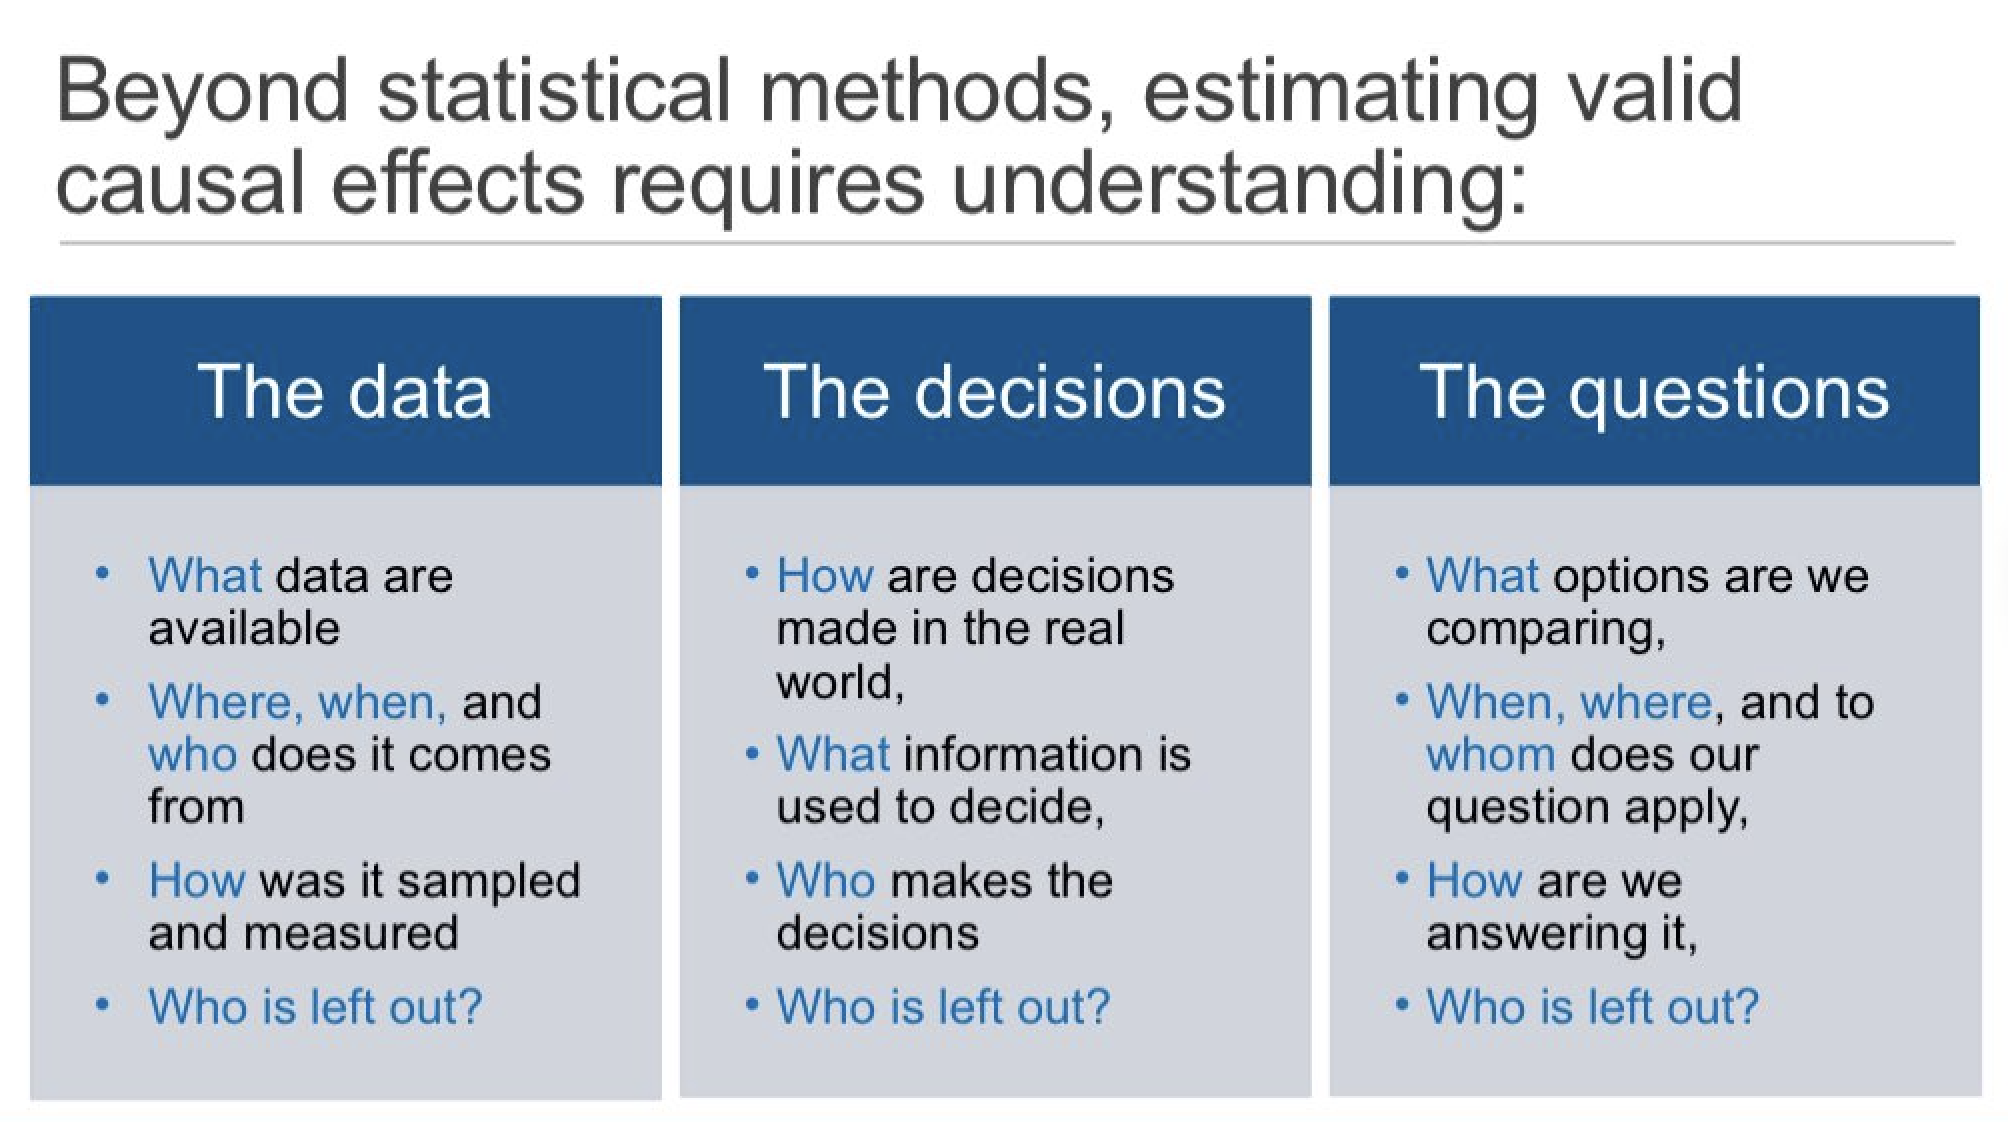
\includegraphics[width=0.75\textwidth,height=\textheight]{chapters/key_notions/../../figures/data_biases.png}

}

\caption{Tabella creata da Ellie Murray.}

\end{figure}%

\subsection{Variabili e Costanti}\label{variabili-e-costanti}

Nell'analisi statistica, le \emph{variabili} rappresentano le
caratteristiche osservate che possono assumere diversi valori (numerici
o categorici). Al contrario, le \emph{costanti} sono valori che
rimangono fissi in un dato contesto. Si distinguono poi le variabili
indipendenti (o predittive), che influenzano le variabili dipendenti, e
le variabili dipendenti, che rappresentano gli esiti di interesse.

\subsection{Effetti}\label{effetti}

In statistica, un \emph{effetto} misura il cambiamento osservato nelle
variabili dipendenti in relazione alle variabili indipendenti. Ad
esempio, l'efficacia di una terapia può essere valutata misurando la
differenza nei sintomi prima e dopo il trattamento
(\citeproc{ref-huntington2021effect}{Huntington-Klein, 2021}).

\subsection{Stima e Inferenza}\label{stima-e-inferenza}

\subsubsection{Stima}\label{stima}

La stima statistica consente di ottenere informazioni su una popolazione
a partire da un campione. Si utilizzano statistiche campionarie (come la
media campionaria) per stimare i parametri della popolazione (come la
media vera della popolazione).

Gli stimatori devono possedere proprietà come:

\begin{itemize}
\tightlist
\item
  consistenza: la stima converge al vero valore del parametro
  all'aumentare della dimensione del campione;
\item
  non distorsione: il valore atteso dello stimatore è uguale al vero
  valore del parametro;
\item
  efficienza: lo stimatore ha la minor varianza possibile.
\end{itemize}

L'accuratezza della stima dipende da vari fattori, tra cui la dimensione
e la rappresentatività del campione, la variabilità nella popolazione e
il metodo di campionamento utilizzato.

\subsection{Inferenza Statistica}\label{inferenza-statistica}

Dopo aver ottenuto le stime, l'inferenza statistica permette di trarre
conclusioni più generali sulla popolazione. Essa consente di valutare
ipotesi specifiche o rispondere a domande di ricerca basate sui dati
raccolti.

Ad esempio, se abbiamo stimato la media del rendimento accademico in un
campione di studenti, l'inferenza statistica ci consente di quantificare
l'incertezza riguardo alla differenza di rendimento tra maschi e femmine
all'interno della popolazione più ampia. In questo modo, l'inferenza
statistica ci fornisce gli strumenti per fare previsioni e trarre
conclusioni su fenomeni che riguardano l'intera popolazione.

Esistono due approcci principali.

\textbf{L'inferenza bayesiana}:

\begin{itemize}
\tightlist
\item
  Si basa sul teorema di Bayes;
\item
  Utilizza probabilità a priori, che riflettono conoscenze o credenze
  iniziali su un fenomeno;
\item
  Aggiorna queste probabilità con nuovi dati per ottenere probabilità a
  posteriori;
\item
  Fornisce una interpretazione delle probabilità come gradi di credenza
  soggettivi.
\end{itemize}

\textbf{L'approccio frequentista}:

\begin{itemize}
\tightlist
\item
  Si fonda sulla frequenza relativa di eventi osservati in esperimenti
  ripetuti;
\item
  Utilizza strumenti come il test di ipotesi nulla e gli intervalli di
  confidenza per trarre conclusioni;
\item
  Non fa uso di probabilità a priori, concentrandosi esclusivamente sui
  dati osservati.
\end{itemize}

\section{Le Sfide dell'Inferenza Statistica in
Psicologia}\label{le-sfide-dellinferenza-statistica-in-psicologia}

Secondo Gelman et al. (\citeproc{ref-gelman2020regression}{2020}),
l'inferenza statistica in psicologia affronta tre sfide principali:

\begin{enumerate}
\def\labelenumi{\arabic{enumi}.}
\item
  \textbf{Generalizzare dai campioni alla popolazione}: Questa sfida è
  strettamente legata al problema del campionamento di comodo, spesso
  usato in psicologia, ma presente in quasi tutte le applicazioni
  dell'inferenza statistica. La difficoltà risiede nel trarre
  conclusioni affidabili su una popolazione più ampia partendo da un
  campione limitato e, a volte, non rappresentativo.
\item
  \textbf{Generalizzare dal gruppo trattato al gruppo di controllo}:
  Questa sfida riguarda l'inferenza causale, un aspetto centrale per
  determinare l'efficacia dei trattamenti psicologici. L'obiettivo è
  stabilire se i risultati osservati nel gruppo trattato possano essere
  applicati al gruppo di controllo o ad altre popolazioni, permettendo
  una valutazione valida dell'effetto del trattamento.
\item
  \textbf{Generalizzare dalle misurazioni osservate ai costrutti
  sottostanti}: In psicologia, i dati raccolti non corrispondono mai
  perfettamente ai costrutti teorici di interesse. La sfida è inferire
  questi costrutti latenti dai dati osservati, che rappresentano spesso
  solo un'approssimazione imperfetta.
\end{enumerate}

Queste sfide evidenziano la complessità dell'inferenza in psicologia e
la necessità di metodologie robuste per affrontarle.

\section{Riflessioni Conclusive}\label{riflessioni-conclusive-1}

In psicologia, le teorie forniscono ipotesi testabili che spiegano il
``come'' e il ``perché'' di determinati fenomeni mentali e
comportamentali. Una teoria robusta permette di formulare previsioni
chiare e specifiche, che possono essere verificate empiricamente
attraverso l'analisi dei dati. Ad esempio, una teoria sull'ansia
potrebbe prevedere che, in un compito di esposizione graduale a stimoli
ansiogeni, il livello di ansia diminuisca progressivamente. Senza una
teoria che spieghi perché questo dovrebbe accadere, tale osservazione
rimane solo un dato descrittivo, privo di valore esplicativo o
predittivo.

L'analisi dei dati diventa davvero potente quando è integrata a una
teoria. Senza teoria, i dati possono descrivere fenomeni ma non spiegare
i meccanismi sottostanti. La teoria fornisce il contesto interpretativo,
orientando la raccolta e l'analisi dei dati, e permettendo una
comprensione profonda dei fenomeni psicologici.

Un esempio è l'uso della data science per analizzare l'efficacia di un
trattamento psicoterapeutico. I dati possono mostrarci una diminuzione
dei sintomi in seguito alla terapia, ma è solo la teoria alla base del
trattamento che fornisce un quadro interpretativo per questo
miglioramento, proponendo i meccanismi per cui il trattamento riduce i
sintomi. La teoria orienta quindi l'analisi e permette di interpretare i
dati in un contesto scientifico.

Sviluppare una teoria in psicologia è complesso a causa della notevole
variabilità umana. Un buon modello psicologico deve prevedere con
precisione i comportamenti osservabili e rappresentare i processi
mentali latenti. Queste previsioni devono essere testabili e
falsificabili (\citeproc{ref-eronen2021theory}{Eronen \& Bringmann,
2021}).

La relazione tra teoria e analisi dei dati è dinamica e iterativa. I
modelli e le teorie si evolvono grazie alla verifica empirica. Se i dati
non supportano le previsioni di una teoria, essa viene modificata o
sostituita, favorendo l'avanzamento scientifico.

In conclusione, la teoria e l'analisi dei dati sono complementari e
interdipendenti. L'analisi dei dati offre gli strumenti per testare e
affinare le teorie psicologiche, mentre la teoria dà significato e
contesto ai dati, rendendo possibile una comprensione profonda e utile
dei fenomeni psicologici.

\section*{Bibliografia}\label{bibliografia-1}
\addcontentsline{toc}{section}{Bibliografia}

\markright{Bibliografia}

\chapter{La misurazione in psicologia}\label{sec-measurement}

\begin{quote}
Measurement, measurement, measurement. It's central to statistics. It's
central to how we learn about the world. (A. Gelman)
\end{quote}

\textbf{Prerequisiti}

\begin{itemize}
\tightlist
\item
  Leggere
  \href{https://www.sciencedirect.com/science/article/pii/S0263224115005801?casa_token=QTLWp2GIWswAAAAA:wmewUxxK68plnyJhu51VMpVSnI4rB5wB36p4l1KlKarbFwhFTuIWUS7V5ZHdfhoqSqiy4JJoqg}{On
  the philosophical foundations of psychological measurement
  (\citeproc{ref-maul2016philosophical}{Maul et al., 2016})} sui
  fondamenti filosofici della misurazione psicologica.
\item
  Leggere
  \href{https://web.p.ebscohost.com/ehost/pdfviewer/pdfviewer?vid=0&sid=52940ed5-6696-4f73-be23-b5f868703f25\%40redis}{Psychological
  Measurement and the Replication Crisis: Four Sacred Cows
  (\citeproc{ref-lilienfeld2020psychological}{Lilienfeld \& Strother,
  2020})}. Questo articolo mette in relazione le proprietà delle misure
  psicologiche con la crisi della replicabilità dei risultati della
  ricerca.
\item
  Leggere la sezione sui numeri dell'\textbf{?@sec-numbers}.
\end{itemize}

\textbf{Concetti e competenze chiave}

\begin{itemize}
\tightlist
\item
  Conoscere le proprietà delle scale di misura di Stevens.
\item
  Comprendere quali operazioni aritmetiche possono essere applicate a
  ciascun livello di scala e perchè.
\item
  Distinguere tra variabili continue e discrete.
\item
  Capire la differenza tra accuratezza e attendibilità.
\item
  Conoscere i diversi tipi di validità e affidabilità.
\end{itemize}

\section{Introduzione}\label{introduzione-3}

La scienza si avvale di modelli per interpretare i dati, ma opera sempre
con teorie incomplete e misurazioni soggette a errori. Di conseguenza, è
fondamentale riconoscere le incertezze quando si cerca di estrarre
informazioni dalle misurazioni utilizzando i nostri modelli. Nessuna
misurazione, spiegazione o previsione è perfettamente accurata e
precisa, e non possiamo mai conoscere con esattezza l'entità dei loro
errori.

Questa incertezza viene catturata in tre equazioni fondamentali. La
prima è l'\emph{Equazione di Misurazione}, che riconosce l'errore
osservativo: \(y = z + ϵ_y\), dove \(y\) rappresenta il valore misurato,
\(z\) il valore reale e \(ϵ_y\) l'errore di misurazione. La seconda è
l'\emph{Equazione di Modellazione}, che esprime la presenza di un
diverso tipo di errore: \(z = f(x,θ) + ϵ_\text{model}\), dove \(f\) è il
modello, \(x\) sono le condizioni ambientali per cui eseguiamo il
modello, θ sono i valori dei parametri del modello e \(ϵ_\text{model}\)
rappresenta l'errore del modello, che sorge perché \(f\), \(x\) e θ
saranno tutti in qualche misura imprecisi.

Combinando queste due equazioni, otteniamo l'\emph{Equazione della
Scienza}: \(y = f(x,θ) + ϵ_\text{model} + ϵ_y\). La scienza è il
tentativo di spiegare le osservazioni \(y\) utilizzando un modello
\(f\), cercando di minimizzare l'errore di misurazione \(ϵ_y\) e
l'errore del modello \(ϵ_\text{model}\), in modo che il modello possa
essere utilizzato per fare previsioni sul mondo reale (\(z\)).
L'approccio bayesiano alla scienza riconosce e quantifica le incertezze
su tutti e sei gli elementi dell'Equazione della Scienza: \(y\), \(f\),
\(x\), θ, \(ϵ_\text{model}\) e \(ϵ_y\).

\section{La teoria della Misurazione}\label{la-teoria-della-misurazione}

La teoria della misurazione, oggetto di questo capitolo, si concentra
sull'errore di misurazione e sull'equazione fondamentale
\(y = z + ϵ_y\). Questa equazione può essere esaminata da tre
prospettive distinte. La prima concerne l'affidabilità della misura,
rappresentata dal termine \(ϵ_y\). La psicometria, branca dedicata alla
teoria della misurazione psicologica, si occupa di quantificare
l'affidabilità delle misure psicologiche attraverso metodi come la
Teoria Classica dei Test e la Teoria di Risposta all'Item.

La seconda prospettiva riguarda la validità delle misure psicologiche,
ovvero quanto adeguatamente la misura \(y\) rappresenti il costrutto
\(z\). Questo aspetto, più complesso dell'affidabilità, non può essere
risolto meramente con metodi statistici, ma richiede una profonda
comprensione delle teorie psicologiche e della loro capacità di
descrivere e prevedere i fenomeni psicologici.

La terza prospettiva si concentra sulle procedure di assegnazione dei
valori a \(y\), esplorando quali metodi (questionari, interviste,
esperimenti) siano più appropriati e come valutarne l'adeguatezza.

\subsection{Costrutti Psicologici}\label{costrutti-psicologici}

La teoria della misurazione sottolinea l'importanza di distinguere tra
la procedura di misurazione e il costrutto che si intende misurare. Ad
esempio, mentre la temperatura è un costrutto, il termometro è lo
strumento di misurazione. Analogamente, l'abilità matematica è un
costrutto, mentre un test di matematica è la procedura per misurarla.

Nelle scienze psicologiche e sociali, la misurazione presenta sfide
uniche rispetto alle scienze fisiche, poiché i costrutti in esame sono
spesso astratti e non direttamente osservabili. Ciò richiede una
particolare attenzione alla validità e all'affidabilità degli strumenti
di misurazione, nonché una costante riflessione sulle limitazioni e le
potenziali fonti di errore.

Il capitolo introduce concetti fondamentali relativi alla misurazione
quantitativa delle caratteristiche psicologiche, con un focus sulla
teoria delle scale di misura di Stevens (1946). Questa teoria fornisce
un quadro concettuale per comprendere i diversi tipi di scale di
misurazione e le operazioni matematiche appropriate per ciascuna.
Inoltre, vengono esplorate alcune procedure di scaling psicologico,
ovvero l'assegnazione di numeri all'intensità di fenomeni psicologici.

\subsection{Scaling Psicologico}\label{scaling-psicologico}

Lo scaling psicologico si occupa della trasformazione dei dati empirici
raccolti durante uno studio psicologico in misure o punteggi che
rappresentino accuratamente le caratteristiche psicologiche oggetto di
indagine.

\textbf{Scaling di Guttman.} Uno dei metodi di scaling più noti è lo
«Scaling di Guttman», che viene utilizzato per rappresentare relazioni
ordinate tra gli elementi di una scala. Ad esempio, in un questionario
sui sintomi dell'ansia, le domande possono essere disposte in ordine di
intensità crescente dei sintomi. Secondo il modello di Guttman, se un
partecipante risponde ``sì'' a una domanda che riflette un sintomo più
intenso, ci si aspetta che abbia risposto ``sì'' anche a tutte le
domande precedenti, che rappresentano sintomi di intensità minore.
Questo approccio consente di costruire una scala che riflette in modo
sistematico e coerente la gravità dei sintomi.

\textbf{Scaling Thurstoniano.} Lo «Scaling Thurstoniano» è un metodo
utilizzato per misurare preferenze o giudizi soggettivi. Ad esempio, per
valutare la preferenza tra diversi tipi di cibi, i partecipanti
confrontano due cibi alla volta ed esprimono una preferenza. Le risposte
vengono poi utilizzate per assegnare punteggi che riflettono la
preferenza media per ciascun cibo.

\textbf{Questionari Likert.} I questionari Likert richiedono ai
partecipanti di esprimere il loro grado di accordo con una serie di
affermazioni su una scala a più livelli, che va da «fortemente in
disaccordo» a «fortemente d'accordo». I punteggi ottenuti vengono
sommati per rappresentare la posizione complessiva dell'individuo
rispetto all'oggetto di studio.

\subsection{Metodi di Valutazione delle Scale
Psicologiche}\label{metodi-di-valutazione-delle-scale-psicologiche}

Per valutare le proprietà delle scale psicologiche, vengono utilizzati
vari metodi. Ad esempio, l'affidabilità delle misure può essere
analizzata utilizzando il coefficiente alpha di Cronbach o il
coefficiente Omega di McDonald, entrambi utilizzati per misurare la
coerenza interna delle risposte ai diversi item di un questionario.
Inoltre, la validità delle scale può essere esaminata confrontando i
risultati ottenuti con misure simili o attraverso analisi statistiche
che verificano se la scala cattura accuratamente il costrutto
psicologico che si intende misurare. La validità di costrutto è
particolarmente cruciale, poiché riguarda la capacità della scala di
misurare effettivamente il concetto psicologico che si intende
esplorare.

\subsection{Prospettive Moderne}\label{prospettive-moderne}

Negli ultimi anni, il dibattito sulla misurazione psicologica si è
arricchito di nuove prospettive, grazie all'avvento di tecnologie
avanzate e all'integrazione di approcci interdisciplinari. Ecco alcune
delle tendenze più rilevanti.

\textbf{Teoria della Risposta agli Item.} La Teoria della Risposta agli
Item (IRT) ha guadagnato popolarità per la sua capacità di fornire stime
più precise delle abilità latenti rispetto ai modelli classici. La IRT
considera la probabilità che un individuo risponda correttamente a un
item in funzione della sua abilità e delle caratteristiche dell'item
stesso, offrendo una visione più dettagliata delle proprietà
psicometriche degli strumenti di misurazione.

\textbf{Approcci Bayesiani.} Gli approcci bayesiani stanno
rivoluzionando il campo della psicometria, permettendo di incorporare
informazioni a priori nelle stime e di aggiornare le credenze sulla base
di nuovi dati. Questi metodi sono particolarmente utili per affrontare
la complessità e l'incertezza inerenti alla misurazione psicologica.

\textbf{Analisi di Rete.} L'analisi di rete è un'altra metodologia
emergente che vede i costrutti psicologici non come variabili latenti
indipendenti, ma come reti di sintomi interconnessi. Questo approccio
può offrire nuove intuizioni sulla struttura delle psicopatologie e
sulla dinamica dei sintomi.

\section{Le scale di misurazione}\label{le-scale-di-misurazione}

Le scale di misurazione sono strumenti fondamentali per assegnare numeri
ai dati osservati, rappresentando le proprietà psicologiche. La teoria
delle scale di Stevens Stevens (\citeproc{ref-stevens_46}{1946})
identifica quattro tipi di scale di misurazione: nominali, ordinali, a
intervalli e di rapporti. Ognuna di queste scale consente di effettuare
operazioni aritmetiche diverse, poiché ciascuna di esse è in grado di
``catturare'' solo alcune delle proprietà dei fenomeni psicologici che
si intende misurare.

\begin{figure}[H]

{\centering 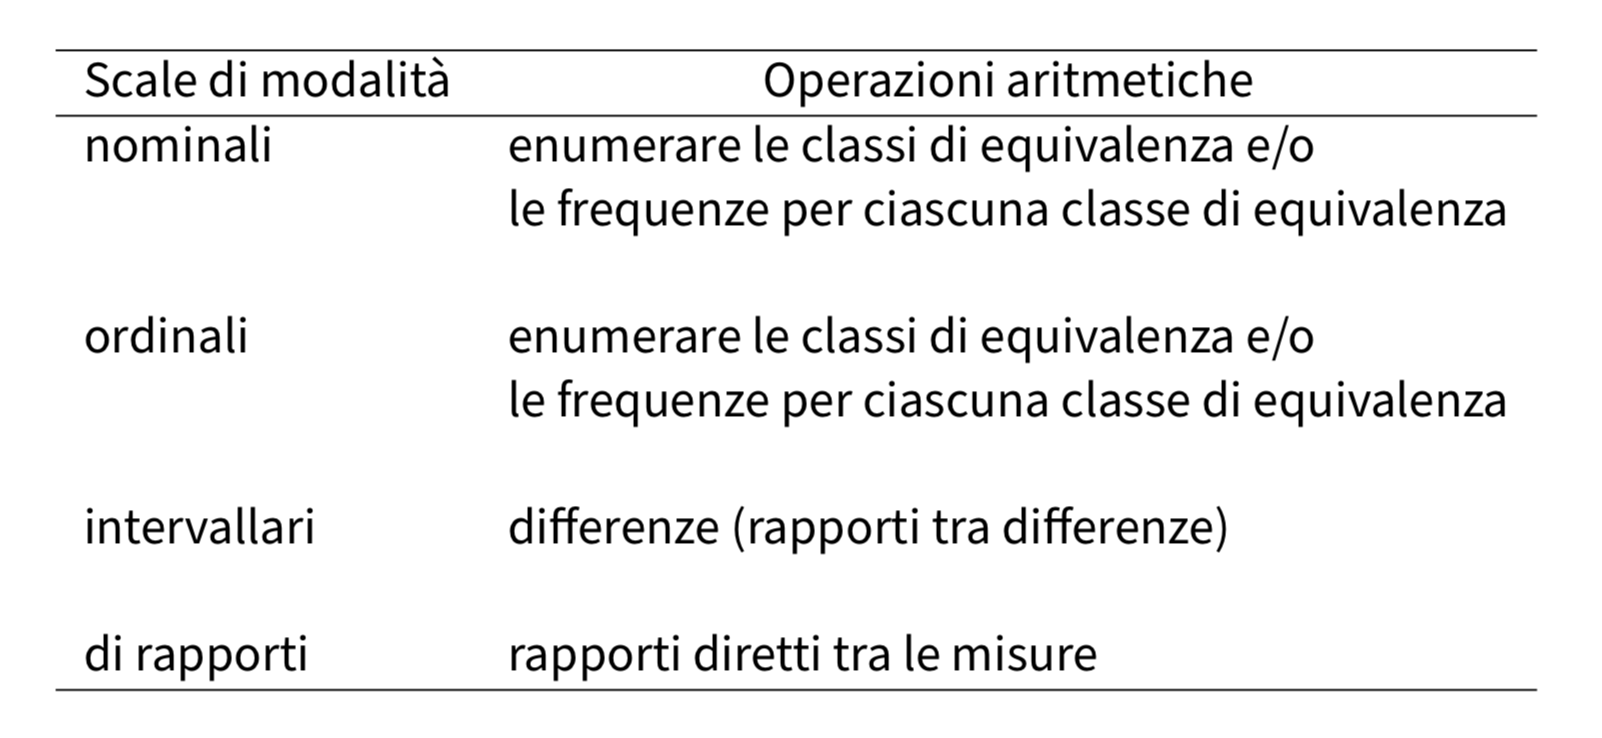
\includegraphics[width=0.7\textwidth,height=\textheight]{chapters/key_notions/../../figures/misurazione_2.png}

}

\caption{Scale di misurazione.}

\end{figure}%

\subsection{Scala nominale}\label{scala-nominale}

ILa scala nominale è il livello di misurazione più semplice e
corrisponde ad una tassonomia o classificazione delle categorie che
utilizziamo per descrivere i fenomeni psicologici. I simboli o numeri
che costituiscono questa scala rappresentano i nomi delle categorie e
non hanno alcun valore numerico intrinseco. Con la scala nominale
possiamo solo distinguere se una caratteristica psicologica è uguale o
diversa da un'altra.

I dati raccolti con la scala nominale sono suddivisi in categorie
qualitative e mutuamente esclusive, in cui ogni dato appartiene ad una
sola categoria. In questa scala, esiste solo la relazione di equivalenza
tra le misure delle unità di studio: gli elementi del campione
appartenenti a classi diverse sono differenti, mentre tutti quelli della
stessa classe sono tra loro equivalenti.

L'unica operazione algebrica consentita dalla scala nominale è quella di
contare le unità di studio che appartengono ad ogni categoria e il
numero totale di categorie. Di conseguenza, la descrizione dei dati
avviene tramite le frequenze assolute e le frequenze relative.

Dalla scala nominale è possibile costruire altre scale nominali
equivalenti alla prima, trasformando i valori della scala di partenza in
modo tale da cambiare i nomi delle categorie, ma lasciando inalterata la
suddivisione delle unità di studio nelle medesime classi di equivalenza.
In altre parole, cambiando i nomi delle categorie di una variabile
misurata su scala nominale, si ottiene una nuova variabile esattamente
equivalente alla prima.

\subsection{Scala ordinale}\label{scala-ordinale}

La scala ordinale mantiene la caratteristica della scala nominale di
classificare ogni unità di misura all'interno di una singola categoria,
ma introduce la relazione di ordinamento tra le categorie. In quanto
basata su una relazione di ordine, una scala ordinale descrive solo il
rango di ordine tra le categorie e non fornisce informazioni sulla
distanza tra di esse. Non ci dice, ad esempio, se la distanza tra le
categorie \(a\) e \(b\) è uguale, maggiore o minore della distanza tra
le categorie \(b\) e \(c\).

Un esempio classico di scala ordinale è quello della scala Mohs per la
determinazione della durezza dei minerali. Per stabilire la durezza dei
minerali si usa il criterio empirico della scalfittura. Vengono
stabiliti livelli di durezza crescente da 1 a 10 con riferimento a dieci
minerali: talco, gesso, calcite, fluorite, apatite, ortoclasio, quarzo,
topazio, corindone e diamante. Un minerale appartenente ad uno di questi
livelli se scalfisce quello di livello inferiore ed è scalfito da quello
di livello superiore.

\begin{figure}[H]

{\centering 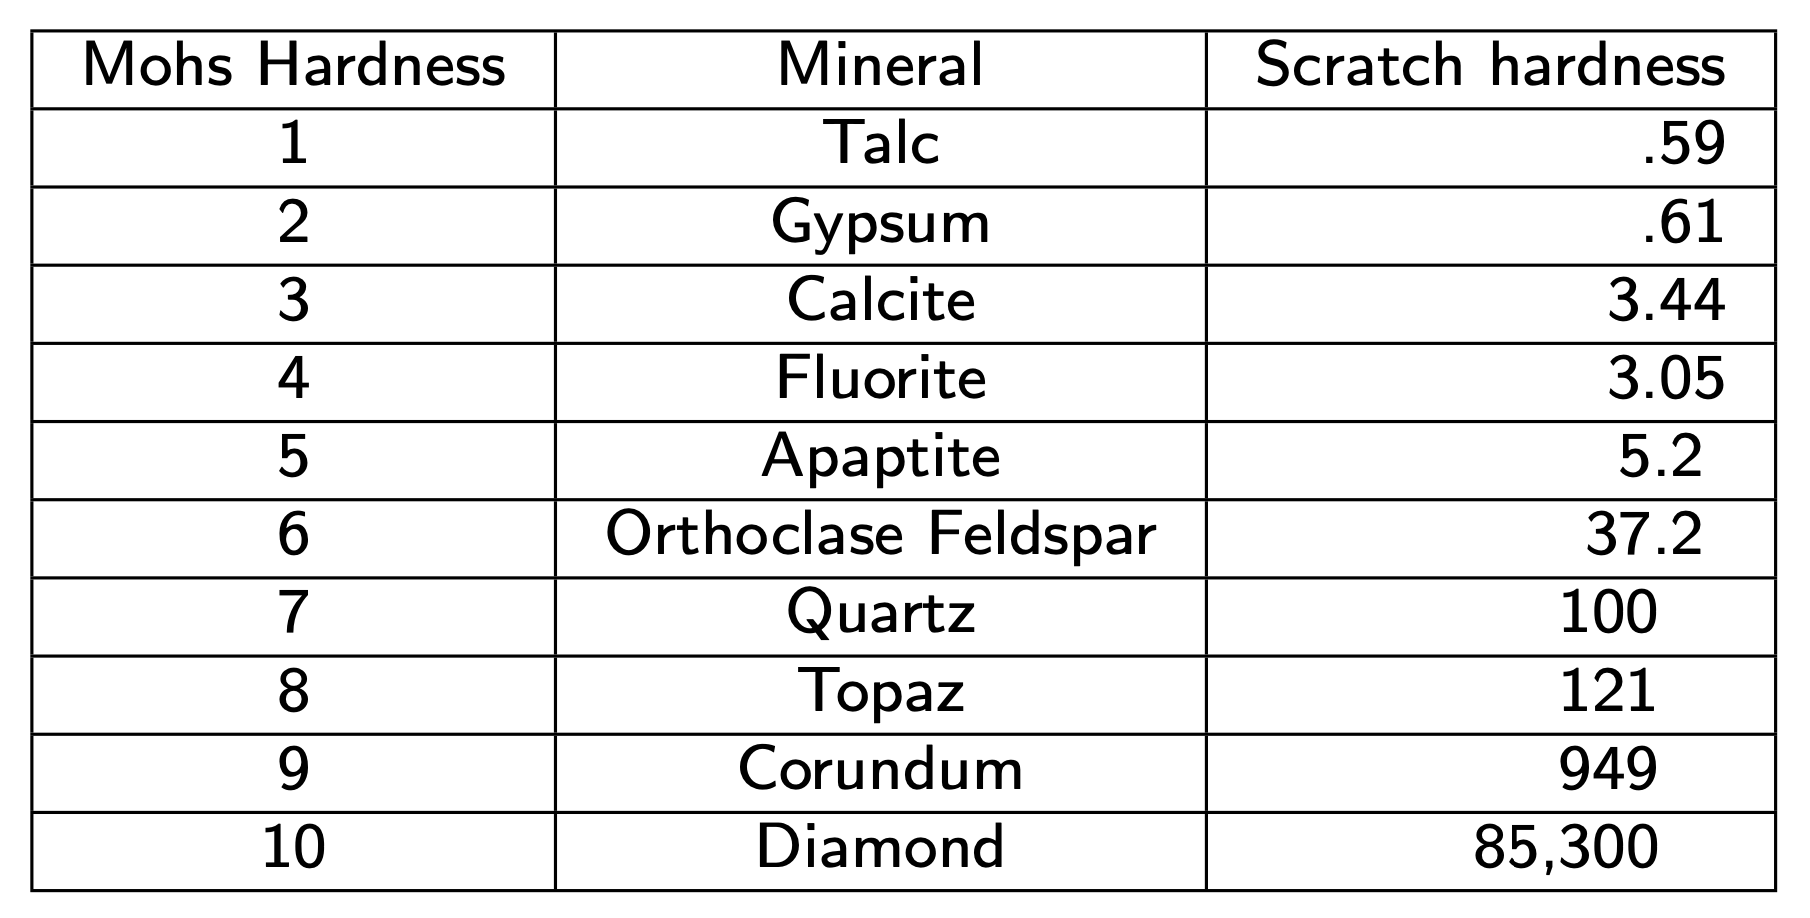
\includegraphics[width=0.62\textwidth,height=\textheight]{chapters/key_notions/../../figures/mohs.png}

}

\caption{La scala di durezza dei minerali di Mohs. Un oggetto è
considerato più duro di X se graffia X. Sono incluse anche misure di
durezza relativa utilizzando uno sclerometro, da cui emerge la non
linearità della scala di Mohs (Burchard, 2004).}

\end{figure}%

\subsection{Scala ad intervalli}\label{scala-ad-intervalli}

La scala ad intervalli di misurazione include le proprietà della scala
nominale e della scala ordinale e permette di misurare le distanze tra
le coppie di unità statistiche in termini di un intervallo costante,
chiamato ``unità di misura'', a cui viene attribuito il valore ``1''.
L'origine della scala, ovvero il punto zero, è scelta arbitrariamente e
non indica l'assenza della proprietà che si sta misurando. Ciò significa
che la scala ad intervalli consente anche valori negativi e lo zero non
viene attribuito all'unità statistica in cui la proprietà risulta
assente.

La scala ad intervalli equivalenti consente l'esecuzione di operazioni
algebriche basate sulla differenza tra i numeri associati ai diversi
punti della scala, operazioni algebriche non possibili con le scale di
misura nominale o ordinale. Tuttavia, il limite della scala ad
intervalli è che non consente di calcolare il rapporto tra coppie di
misure. È possibile affermare la differenza tra \(a\) e \(b\) come la
metà della differenza tra \(c\) e \(d\) o che le due differenze sono
uguali, ma non è possibile affermare che \(a\) abbia una proprietà
misurata in quantità doppia rispetto a \(b\). In altre parole, non è
possibile stabilire rapporti diretti tra le misure ottenute. Solo le
differenze tra le modalità permettono tutte le operazioni aritmetiche,
come la somma, l'elevazione a potenza o la divisione, che sono alla base
della statistica inferenziale.

Nelle scale ad intervalli equivalenti, l'unità di misura è arbitraria e
può essere cambiata attraverso una dilatazione, ovvero la
moltiplicazione di tutti i valori della scala per una costante positiva.
Inoltre, la traslazione, ovvero l'aggiunta di una costante a tutti i
valori della scala, è ammessa poiché non altera le differenze tra i
valori della scala. La scala rimane invariata rispetto a traslazioni e
dilatazioni e dunque le uniche trasformazioni ammissibili sono le
trasformazioni lineari:

\[
y' = a + by, \quad b > 0.
\]

Infatti, l'uguaglianza dei rapporti fra gli intervalli rimane invariata
a seguito di una trasformazione lineare.

Esempio di scala ad intervalli è la temperatura misurata in gradi
Celsius o Fahrenheit, ma non Kelvin. Come per la scala nominale, è
possibile stabilire se due modalità sono uguali o diverse: 30\(^\circ\)C
\(\neq\) 20\(^\circ\)C. Come per la scala ordinale è possibile mettere
due modalità in una relazione d'ordine: 30\(^\circ\)C \(>\)
20\(^\circ\)C. In aggiunta ai casi precedenti, però, è possibile
definire una unità di misura per cui è possibile dire che tra
30\(^\circ\)C e 20\(^\circ\)C c'è una differenza di 30\(^\circ\) -
20\(^\circ\) = 10\(^\circ\)C. I valori di temperatura, oltre a poter
essere ordinati secondo l'intensità del fenomeno, godono della proprietà
che le differenze tra loro sono direttamente confrontabili e
quantificabili.

Il limite della scala ad intervalli è quello di non consentire il
calcolo del rapporto tra coppie di misure. Ad esempio, una temperatura
di 80\(^\circ\)C non è il doppio di una di 40\(^\circ\)C. Se infatti
esprimiamo le stesse temperature nei termini della scala Fahrenheit,
allora i due valori non saranno in rapporto di 1 a 2 tra loro. Infatti,
20\(^\circ\)C = 68\(^\circ\)F e 40\(^\circ\)C = 104\(^\circ\)F. Questo
significa che la relazione ``il doppio di'' che avevamo individuato in
precedenza si applicava ai numeri della scala centigrada, ma non alla
proprietà misurata (cioè la temperatura). La decisione di che scala
usare (Centigrada vs.~Fahrenheit) è arbitraria. Ma questa arbitrarietà
non deve influenzare le inferenze che traiamo dai dati. Queste
inferenze, infatti, devono dirci qualcosa a proposito della realtà
empirica e non possono in nessun modo essere condizionate dalle nostre
scelte arbitrarie che ci portano a scegliere la scala Centigrada
piuttosto che quella Fahrenheit.

Consideriamo ora l'aspetto invariante di una trasformazione lineare,
ovvero l'uguaglianza dei rapporti fra intervalli. Prendiamo in esame, ad
esempio, tre temperature: \(20^\circ C = 68^\circ F\),
\(15^\circ C = 59^\circ F\), \(10^\circ C = 50 ^\circ F\).

È facile rendersi conto del fatto che i rapporti fra intervalli restano
costanti indipendentemente dall'unità di misura che è stata scelta:

\[
  \frac{20^\circ C - 10^\circ C}{20^\circ C - 15^\circ C} =
  \frac{68^\circ F - 50^\circ F}{68^\circ F-59^\circ F} = 2.
\]

\subsection{Scala di rapporti}\label{scala-di-rapporti}

Nella scala a rapporti equivalenti, lo zero non è arbitrario e
rappresenta l'elemento che ha intensità nulla rispetto alla proprietà
misurata. Per costruire questa scala, si associa il numero 0
all'elemento con intensità nulla e si sceglie un'unità di misura \(u\).
Ad ogni elemento si assegna un numero \(a\) definito come \(a=d/u\),
dove \(d\) rappresenta la distanza dall'origine. In questo modo, i
numeri assegnati riflettono le differenze e i rapporti tra le intensità
della proprietà misurata.

In questa scala, è possibile effettuare operazioni aritmetiche non solo
sulle differenze tra i valori della scala, ma anche sui valori stessi
della scala. L'unica scelta arbitraria è l'unità di misura, ma lo zero
deve sempre rappresentare l'intensità nulla della proprietà considerata.

Le trasformazioni ammissibili in questa scala sono chiamate
trasformazioni di similarità e sono del tipo \(y' = by\), dove \(b>0\).
In questa scala, i rapporti tra i valori rimangono invariati dopo le
trasformazioni. In altre parole, se rapportiamo due valori originali e
due valori trasformati, il rapporto rimane lo stesso:
\(\frac{y_i}{y_j} = \frac{y'_i}{y'_j}\).

\section{Gerarchia dei livelli delle scale di
misurazione}\label{gerarchia-dei-livelli-delle-scale-di-misurazione}

Secondo Stevens (\citeproc{ref-stevens_46}{1946}), esiste una gerarchia
dei livelli delle scale di misurazione, denominati ``livelli di scala''.
Questi livelli sono organizzati in modo gerarchico, in cui la scala
nominale rappresenta il livello più basso della misurazione, mentre la
scala a rapporti equivalenti rappresenta il livello più alto.

\begin{itemize}
\tightlist
\item
  La scala nominale è il livello più elementare, in cui le categorie o
  le etichette vengono assegnate agli oggetti o agli individui senza
  alcuna valutazione di grandezza o ordine.
\item
  Al livello successivo si trova la scala ordinale, in cui le categorie
  sono ordinate in base a una qualche qualità o caratteristica. Qui, è
  possibile stabilire un ordine di preferenza o gerarchia tra le
  categorie, ma non è possibile quantificare la differenza tra di esse
  in modo preciso.
\item
  La scala intervallo rappresenta un livello successivo, in cui le
  categorie sono ordinate e la differenza tra di esse è quantificabile
  in modo preciso. In questa scala, è possibile effettuare operazioni
  matematiche come l'addizione e la sottrazione tra i valori, ma non è
  possibile stabilire un vero e proprio punto zero significativo.
\item
  Infine, la scala a rapporti equivalenti rappresenta il livello più
  alto. In questa scala, le categorie sono ordinate, la differenza tra
  di esse è quantificabile in modo preciso e esiste un punto zero
  assoluto che rappresenta l'assenza totale della grandezza misurata.
  Questo livello di scala permette di effettuare tutte le operazioni
  matematiche, compresa la moltiplicazione e la divisione.
\end{itemize}

Passando da un livello di misurazione ad uno più alto aumenta il numero
di operazioni aritmetiche che possono essere compiute sui valori della
scala, come indicato nella figura seguente.

\begin{figure}[H]

{\centering 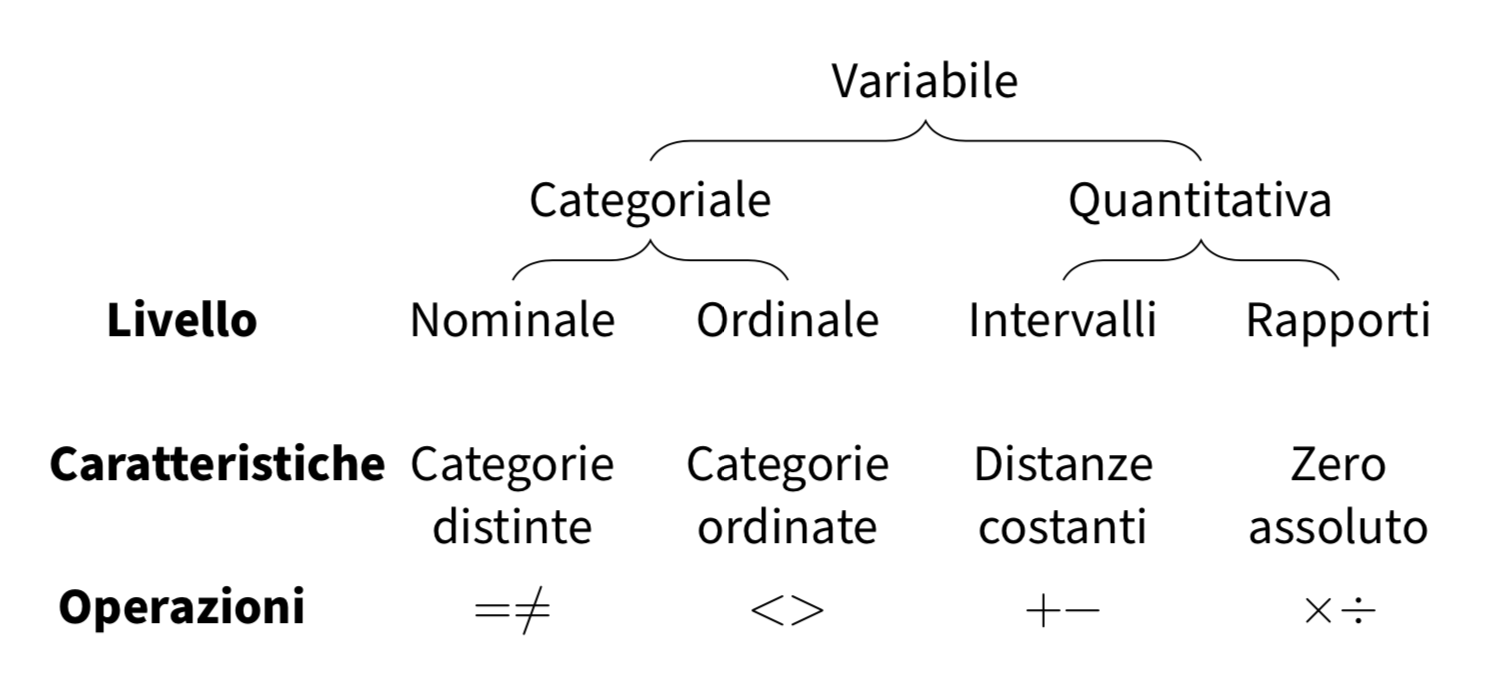
\includegraphics[width=0.65\textwidth,height=\textheight]{chapters/key_notions/../../figures/misurazione_1.png}

}

\caption{Relazioni tra i livelli di misurazione.}

\end{figure}%

Per ciò che riguarda le trasformazioni ammissibili, più il livello di
scala è basso, più le funzioni sono generali (sono minori cioè i vincoli
per passare da una rappresentazione numerica ad un'altra equivalente).
Salendo la gerarchia, la natura delle funzioni di trasformazione si fa
più restrittiva.

\section{Variabili discrete o
continue}\label{variabili-discrete-o-continue}

Le variabili possono essere classificate come variabili a livello di
intervalli o di rapporti e possono essere sia discrete che continue.

\begin{itemize}
\tightlist
\item
  Le variabili discrete assumono valori specifici ma non possono
  assumere valori intermedi. Una volta che l'elenco dei valori
  accettabili è stato definito, non vi sono casi che si trovano tra
  questi valori. In genere, le variabili discrete assumono valori
  interi, come il numero di eventi, il numero di persone o il numero di
  oggetti.
\item
  D'altra parte, le variabili continue possono assumere qualsiasi valore
  all'interno di un intervallo specificato. Teoricamente, ciò significa
  che è possibile utilizzare frazioni e decimali per ottenere qualsiasi
  grado di precisione.
\end{itemize}

\begin{figure}[H]

{\centering 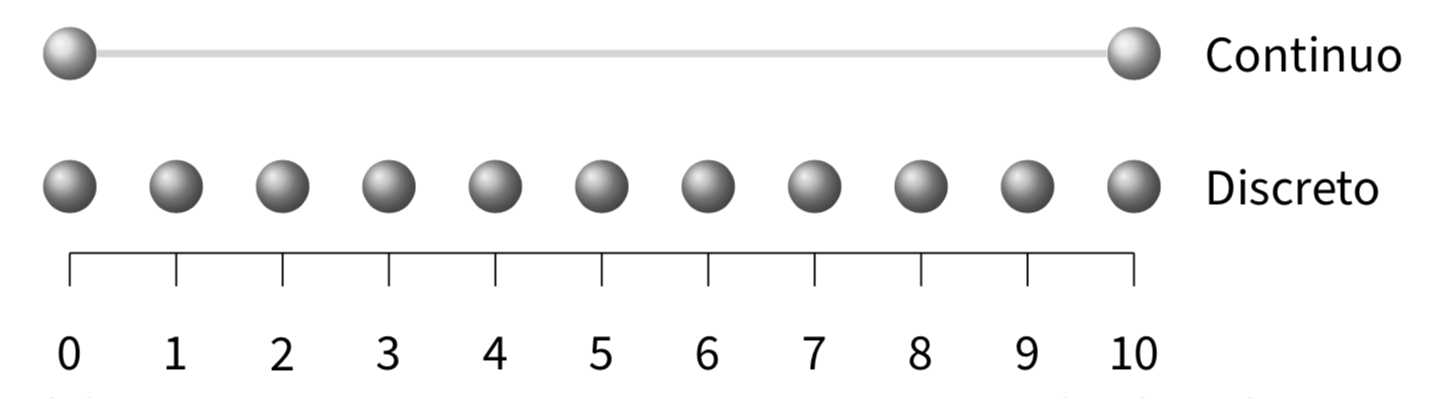
\includegraphics[width=0.65\textwidth,height=\textheight]{chapters/key_notions/../../figures/misurazione_3.png}

}

\caption{Variabili discrete e continue.}

\end{figure}%

\section{Comprendere gli errori nella
misurazione}\label{comprendere-gli-errori-nella-misurazione}

Gli errori di misurazione possono essere casuali o sistematici. Gli
errori casuali sono fluttuazioni aleatorie, mentre gli errori
sistematici sono costanti e derivano da problemi nel metodo di
misurazione o negli strumenti.

\subsection{Precisione e Accuratezza}\label{precisione-e-accuratezza}

La precisione indica la coerenza tra misurazioni ripetute, mentre
l'accuratezza si riferisce alla vicinanza del valore misurato al valore
reale. Entrambi i concetti sono cruciali per l'assessment psicometrico.

Utilizzando l'analogia del tiro al bersaglio, si può avere una serie di
colpi vicini tra loro ma lontani dal centro (precisione senza
accuratezza) oppure colpi distribuiti in modo sparso ma in media vicini
al centro (accuratezza senza precisione).

\section{Assessment psicometrico}\label{assessment-psicometrico}

L'assessment psicometrico valuta la qualità delle misurazioni
psicologiche, considerando la validità e l'affidabilità.

\subsection{Validità nella Misurazione
Psicologica}\label{validituxe0-nella-misurazione-psicologica}

La validità è una proprietà psicometrica fondamentale dei test
psicologici. Secondo gli \emph{Standards for Educational and
Psychological Testing} (2014), la validità si riferisce al grado in cui
evidenza e teoria supportano le interpretazioni dei punteggi dei test
per gli usi proposti. Questo concetto evidenzia che la validità riguarda
sia il significato dei punteggi sia il loro utilizzo, rendendola ``la
considerazione più fondamentale nello sviluppo e nella valutazione dei
test''.

\subsection{Evoluzione del Concetto di
Validità}\label{evoluzione-del-concetto-di-validituxe0}

Tradizionalmente, la validità era suddivisa in tre categorie:

\begin{itemize}
\tightlist
\item
  \textbf{Validità di Contenuto}: Si riferisce alla corrispondenza tra
  il contenuto degli item di un test e il dominio dell'attributo
  psicologico che il test intende misurare. È importante che gli item
  siano pertinenti e rappresentativi dell'attributo misurato.
\item
  \textbf{Validità di Criterio}: Valuta il grado di concordanza tra i
  risultati ottenuti tramite lo strumento di misurazione e i risultati
  ottenuti da altri strumenti che misurano lo stesso costrutto o da un
  criterio esterno. Include validità concorrente e predittiva.
\item
  \textbf{Validità di Costrutto}: Riguarda il grado in cui un test
  misura effettivamente il costrutto che si intende misurare. Si
  suddivide in validità convergente (accordo con strumenti che misurano
  lo stesso costrutto) e validità divergente (capacità di discriminare
  tra costrutti diversi).
\end{itemize}

La moderna teoria della validità non adotta più questa visione
tripartita. Gli Standards del 2014 descrivono la validità come un
concetto unitario, dove diverse forme di evidenza concorrono a
supportare l'interpretazione dei punteggi del test per il loro utilizzo
previsto.

\subsection{Tipologie di Prove di
Validità}\label{tipologie-di-prove-di-validituxe0}

Gli Standards del 2014 identificano cinque categorie principali di prove
di validità:

\begin{enumerate}
\def\labelenumi{\arabic{enumi}.}
\tightlist
\item
  \textbf{Prove Basate sul Contenuto del Test}: Valutano quanto il
  contenuto del test rappresenti adeguatamente il dominio del costrutto
  da misurare.
\item
  \textbf{Prove Basate sui Processi di Risposta}: Analizzano se i
  processi cognitivi e comportamentali degli esaminandi riflettono il
  costrutto valutato.
\item
  \textbf{Prove Basate sulla Struttura Interna}: Esaminano la coerenza
  tra gli elementi del test e la struttura teorica del costrutto.
  L'analisi fattoriale è uno strumento chiave in questo contesto.
\item
  \textbf{Prove Basate sulle Relazioni con Altre Variabili}: Studiano la
  correlazione tra i punteggi del test e altre variabili teoricamente
  correlate, utilizzando metodi come la validità convergente e
  divergente.
\item
  \textbf{Prove Basate sulle Conseguenze del Test}: Considerano le
  implicazioni e gli effetti dell'uso del test, sia intenzionali che non
  intenzionali.
\end{enumerate}

\subsection{Minacce alla Validità}\label{minacce-alla-validituxe0}

La validità può essere compromessa quando un test non misura
integralmente il costrutto di interesse (sotto-rappresentazione del
costrutto) o quando include varianza estranea al costrutto. Inoltre,
fattori esterni come l'ansia o la bassa motivazione degli esaminandi, e
deviazioni nelle procedure di amministrazione e valutazione, possono
influenzare negativamente la validità delle interpretazioni dei
risultati.

\subsection{Integrazione delle Prove di
Validità}\label{integrazione-delle-prove-di-validituxe0}

La validità di un test si costruisce attraverso l'integrazione di
diverse linee di evidenza. Ogni interpretazione o uso di un test deve
essere validato specificamente, richiedendo una valutazione continua e
accurata delle prove disponibili. Questo processo implica la costruzione
di un argomento di validità che consideri attentamente la qualità
tecnica del test e l'adeguatezza delle sue interpretazioni per gli scopi
previsti.

In conclusione, la validità è un concetto complesso e integrato che
richiede un'analisi continua e multidimensionale delle evidenze. La
moderna teoria della validità enfatizza l'importanza di considerare
diverse forme di evidenza per supportare le interpretazioni dei punteggi
dei test, garantendo che siano utilizzati in modo appropriato e
significativo. Gli sviluppatori e gli utilizzatori di test devono
impegnarsi a valutare costantemente la validità per assicurare
misurazioni psicologiche accurate e affidabili.

\subsection{Affidabilità}\label{affidabilituxe0}

L'affidabilità concerne la consistenza e stabilità delle misurazioni,
verificata attraverso metodi come l'affidabilità test-retest,
inter-rater, intra-rater e l'affidabilità interna.

\begin{itemize}
\item
  \textbf{Affidabilità Test-Retest}: Questa forma di affidabilità
  verifica la consistenza delle misurazioni nel tempo. Se un individuo
  viene testato in due momenti diversi, i risultati dovrebbero essere
  simili, assumendo che non ci siano stati cambiamenti significativi nel
  costrutto misurato.
\item
  \textbf{Affidabilità Inter-rater}: In questo caso, l'affidabilità è
  determinata dalla concordanza tra le valutazioni di diversi
  esaminatori. Ad esempio, se più psicologi dovessero valutare un
  individuo utilizzando lo stesso strumento, le loro valutazioni
  dovrebbero essere simili.
\item
  \textbf{Affidabilità Intra-rater}: Questa misura dell'affidabilità si
  riferisce alla consistenza delle valutazioni dello stesso esaminatore
  in momenti diversi.
\item
  \textbf{Affidabilità Interna}: Si riferisce alla coerenza delle
  risposte all'interno dello stesso test. Ad esempio, se un test misura
  un costrutto come l'ansia, gli item che misurano l'ansia dovrebbero
  correlare positivamente l'uno con l'altro. Un modo comune per valutare
  l'affidabilità interna è utilizzare il coefficiente \(\omega\) di
  McDonald.
\end{itemize}

\section{Commenti e considerazioni
finali}\label{commenti-e-considerazioni-finali}

La teoria della misurazione è fondamentale nella ricerca empirica per
valutare l'attendibilità e la validità delle misurazioni. È cruciale
valutare l'errore nella misurazione per garantire la precisione e
l'accuratezza delle misure. L'assessment psicometrico si occupa di
valutare la qualità delle misurazioni psicologiche, considerando
l'affidabilità e la validità per garantire misure accurate dei costrutti
teorici. Le moderne tecnologie e metodologie stanno continuamente
arricchendo questo campo, offrendo strumenti sempre più raffinati per la
comprensione delle caratteristiche psicologiche.

\section*{Bibliografia}\label{bibliografia-2}
\addcontentsline{toc}{section}{Bibliografia}

\markright{Bibliografia}

\chapter{L'analisi dei dati psicologici}\label{sec-data-science}

\textbf{Prerequisiti}

\begin{itemize}
\tightlist
\item
  Leggi \emph{Statistical Rethinking}
  (\citeproc{ref-McElreath_rethinking}{McElreath, 2020}). Focalizzati
  sui primi capitoli dove si discute della dicotomia tra ``small world''
  e ``big world''.
\item
  Leggi
  \href{https://statmodeling.stat.columbia.edu/2016/09/21/what-has-happened-down-here-is-the-winds-have-changed/}{What
  has happened down here is the winds have changed (Gelman 2016)}. Un
  post sul blog di Andrew Gelman che fornisce una panoramica sulla crisi
  di replicazione e su come le scienze sociali sono cambiate di
  conseguenza.
\item
  Leggi
  \href{https://psycnet.apa.org/fulltext/2025-04988-001.html}{Productive
  Explanation: A Framework for Evaluating Explanations in Psychological
  Science}. L'adozione di teorie formali è essenziale per affrontare la
  crisi di riproducibilità dei risultati nella ricerca psicologica.
\item
  Per chi è interessato a un romanzo su questi temi, sorprendentemente
  avvincente, consiglio \emph{Quando abbiamo smesso di capire il mondo}
  di Benjamín Labatut (\citeproc{ref-labatut2021abbiamo}{Labatut,
  2021}).
\end{itemize}

\textbf{Concetti e competenze chiave}

\begin{itemize}
\tightlist
\item
  Emergere di ``Credibility Revolution'', ``Causal Revolution'' e
  ``Replication Crisis'' come cambiamento paradigmatico.
\item
  Proliferazione di falsi positivi, p-hacking, campioni
  sottodimensionati e mancanza di trasparenza.
\item
  Paradigma statistico che enfatizza l'aggiornamento delle priors e
  fornisce un framework flessibile per l'inferenza causale.
\item
  Interesse rinnovato nella verifica e sviluppo di modelli che superano
  la mera descrizione delle associazioni tra variabili.
\item
  Precisione, robustezza e rilevanza empirica come standard per le
  spiegazioni teoriche in psicologia.
\end{itemize}

\section*{Introduzione}\label{introduzione-4}
\addcontentsline{toc}{section}{Introduzione}

\markright{Introduzione}

Nel panorama contemporaneo delle scienze sociali e della psicologia, gli
ultimi due decenni hanno visto l'emergere di una profonda trasformazione
metodologica ed epistemologica. Questo movimento, caratterizzato da
concetti chiave quali ``Credibility Revolution''
(\citeproc{ref-angrist2010credibility}{Angrist \& Pischke, 2010}),
``Causal Revolution'' (\citeproc{ref-pearl2018book}{Pearl \& Mackenzie,
2018}) e ``Replication Crisis''
(\citeproc{ref-open2015estimating}{Collaboration, 2015}), ha determinato
un cambiamento paradigmatico nelle pratiche delle scienze sociali e, in
particolare, della psicologia
(\citeproc{ref-korbmacher2023replication}{Korbmacher et al., 2023}).
Questa transizione verso quella che Munger
(\citeproc{ref-munger2023temporal}{2023}) definisce ``Science versione
2'' è stata motivata dalle lacune metodologiche precedenti e ha
catalizzato l'adozione di approcci più rigorosi e replicabili.

La genesi di questa Riforma è radicata nella constatazione di
problematiche metodologiche pervasive, tra cui la proliferazione di
falsi positivi (\citeproc{ref-simmons2011false}{Simmons et al., 2011}),
l'abuso dei ``gradi di libertà dei ricercatori''
(\citeproc{ref-gelman2013garden}{Gelman \& Loken, 2013}), e
l'inadeguatezza delle pratiche statistiche tradizionali
(\citeproc{ref-gelman2014statistical}{Gelman \& Loken, 2014}). Fenomeni
come il p-hacking, l'uso di campioni sottodimensionati
(\citeproc{ref-button2013power}{Button et al., 2013}), e la mancanza di
trasparenza nei metodi di ricerca hanno contribuito a minare la
credibilità delle scoperte psicologiche
(\citeproc{ref-ioannidis2005most}{Ioannidis, 2005};
\citeproc{ref-meehl1967theory}{Meehl, 1967}), portando alla cosiddetta
``Replication Crisis'' (\citeproc{ref-baker20161}{Baker, 2016};
\citeproc{ref-bishop2019psychology}{Bishop, 2019}) -- si veda il
\textbf{?@sec-crisis}.

\section{L'Approccio Bayesiano}\label{lapproccio-bayesiano}

In risposta a queste sfide, l'approccio bayesiano è emerso come un
paradigma statistico fondamentale nella ``Credibility Revolution''.
Contrariamente all'inferenza frequentista basata sul Test dell'Ipotesi
Nulla, la statistica bayesiana offre un framework più flessibile e
intuitivo per l'analisi dei dati e l'inferenza causale. Il principio
cardine dell'approccio bayesiano, l'aggiornamento delle distribuzioni di
probabilità a priori (priors) alla luce di nuove evidenze, si allinea
perfettamente con l'obiettivo di una scienza cumulativa e
auto-correttiva.

L'adozione di metodi bayesiani in psicologia comporta diversi vantaggi
significativi:

\begin{enumerate}
\def\labelenumi{\arabic{enumi}.}
\tightlist
\item
  Quantificazione dell'incertezza: L'inferenza bayesiana fornisce
  distribuzioni di probabilità posteriori complete per i parametri di
  interesse, offrendo una rappresentazione più ricca e sfumata
  dell'incertezza rispetto agli intervalli di confidenza frequentisti.
\item
  Incorporazione di conoscenze pregresse: Le priors bayesiane consentono
  l'integrazione formale di conoscenze precedenti nel processo
  inferenziale, promuovendo un approccio cumulativo alla ricerca.
\item
  Robustezza alle pratiche di ricerca discutibili: I metodi bayesiani
  sono meno suscettibili a pratiche come il p-hacking, poiché
  l'inferenza si basa sull'intera distribuzione posteriore piuttosto che
  su soglie arbitrarie di significatività.
\end{enumerate}

\section{L'approccio bayesiano nella
ricerca}\label{lapproccio-bayesiano-nella-ricerca}

L'impiego delle statistiche bayesiane nella ricerca psicologica presenta
notevoli vantaggi rispetto ad altri metodi statistici tradizionali, come
il test di significatività dell'ipotesi nulla. Un punto di forza
importante risiede nella sua indipendenza dalla teoria dei grandi
campioni, rendendolo particolarmente adatto per gli studi psicologici
che spesso si basano su campioni di dimensioni ridotte
(\citeproc{ref-larson2023bayesian}{Larson et al., 2023}).

La ricerca psicologica è frequentemente caratterizzata da campioni
limitati, dovuti a diversi fattori quali la bassa prevalenza di
determinate condizioni, le difficoltà nel reclutamento dei partecipanti
e le complessità nelle procedure di valutazione. Questi campioni di
piccole dimensioni sono intrinsecamente soggetti a una maggiore
eterogeneità, che si manifesta nella variabilità del fenotipo
comportamentale delle condizioni psicologiche esaminate e nella
discrepanza tra le stime degli effetti in diversi studi. Tale
eterogeneità può condurre a stime degli effetti distorte e scarsamente
riproducibili.

L'approccio bayesiano offre una soluzione efficace a queste
problematiche. In primo luogo, consente di valutare l'adeguatezza della
dimensione del campione attraverso un'analisi della sensibilità dei
risultati rispetto alla specificazione delle distribuzioni a priori. In
secondo luogo, permette di ottenere risultati precisi anche con campioni
ridotti, a condizione che le conoscenze a priori siano accurate e ben
definite.

Un ulteriore vantaggio dell'approccio bayesiano è la sua capacità di
ottimizzare l'uso dei campioni di partecipanti, favorendo un'inclusione
equa delle popolazioni diversificate. Questo è particolarmente rilevante
per gruppi spesso sottorappresentati, come le minoranze etniche. Le
statistiche bayesiane aiutano a superare questa sfida evitando di
esercitare una pressione eccessiva su questi gruppi per aumentarne la
partecipazione, permettendo così una ricerca più equa e rappresentativa.

\section{Modellazione Formale}\label{modellazione-formale}

La ``Credibility Revolution'' ha catalizzato l'integrazione della Data
Science nelle pratiche di ricerca psicologica. L'adozione di pipeline di
analisi dei dati riproducibili, l'uso di controllo di versione, e la
condivisione di dati e codice sono diventati standard de facto nella
comunità scientifica. Questi strumenti non solo migliorano la
trasparenza e la replicabilità della ricerca, ma facilitano anche la
collaborazione e l'accumulo di conoscenze nel campo.

Parallelamente, si è osservato un rinnovato interesse per la
modellazione formale in psicologia, che consente non solo la verifica ma
anche lo sviluppo di modelli dei meccanismi sottostanti ai fenomeni
psicologici (\citeproc{ref-oberauer2019addressing}{Oberauer \&
Lewandowsky, 2019}; \citeproc{ref-van2024productive}{Van Dongen et al.,
2024}). Questo approccio supera la mera descrizione delle associazioni
tra variabili, che era tipica della pratica dominante dell'ANOVA nel
contesto pre-riforma.

La modellazione bayesiana si presta particolarmente bene a questo
approccio, offrendo un framework unificato per la specificazione di
modelli formali, l'incorporazione di incertezza parametrica, e la
valutazione dell'evidenza empirica. Attraverso tecniche come il
confronto tra modelli bayesiano e l'analisi di sensibilità, i
ricercatori possono valutare rigorosamente la plausibilità relativa di
diverse teorie psicologiche.

\section{Riflessioni Epistemologiche}\label{riflessioni-epistemologiche}

L'adozione di metodi bayesiani e della Data Science in psicologia deve
essere accompagnata da una profonda riflessione epistemologica. Come
sottolineato da George Box

\begin{quote}
tutti i modelli sono sbagliati, ma alcuni sono utili.
\end{quote}

Questa massima risuona particolarmente nel contesto della ricerca
psicologica, dove i fenomeni di interesse sono spesso complessi e
multifattoriali.

L'approccio bayesiano, con la sua enfasi sull'aggiornamento iterativo
delle credenze alla luce di nuove evidenze, si allinea naturalmente con
una visione della scienza come processo di apprendimento continuo
piuttosto che come ricerca di verità assolute. Questa prospettiva
riconosce i limiti intrinseci dei nostri modelli e delle nostre teorie,
pur valorizzandone l'utilità euristica e predittiva (si veda la
discussione nella \textbf{?@sec-poetic-validity}).

In particolare, McElreath (\citeproc{ref-McElreath_rethinking}{2020})
sottolinea l'importanza di riconoscere la dualità tra il ``mondo del
modello'' e il mondo reale più ampio che cerchiamo di comprendere.
Questa consapevolezza è cruciale per evitare la reificazione dei nostri
modelli statistici e per mantenere una prospettiva critica sulle nostre
inferenze.

\section{Conclusione}\label{conclusione}

L'integrazione dell'approccio bayesiano e della data science nella
ricerca psicologica rappresenta una risposta promettente alle sfide
poste dalla ``Replication Crisis''. Offrendo un framework coerente per
la modellazione formale, l'inferenza statistica e l'incorporazione di
conoscenze pregresse, questi approcci promettono di elevare il rigore e
la credibilità della ricerca psicologica. Tuttavia, è fondamentale che
l'adozione di questi metodi sia accompagnata da una adeguata
consapevolezza metodologica ed epistemologica -- si veda, ad esempio, il
\textbf{?@sec-causal-inference-regr}.

\section*{Bibliografia}\label{bibliografia-3}
\addcontentsline{toc}{section}{Bibliografia}

\markright{Bibliografia}

\part{EDA}

\chapter*{Introduzione}\label{introduzione-5}
\addcontentsline{toc}{chapter}{Introduzione}

\markboth{Introduzione}{Introduzione}

Dopo aver acquisito un dataset, è fondamentale comprendere a fondo le
caratteristiche dei dati in esso contenuti. Sebbene le statistiche
descrittive e altre misure numeriche siano spesso efficaci per ottenere
una visione d'insieme, talvolta è un'immagine a valere più di mille
parole.

In questa sezione della dispensa, esploreremo alcuni concetti chiave
della statistica descrittiva. Oltre a fornire definizioni teoriche,
presenteremo istruzioni pratiche in Python per condurre analisi
statistiche su dati reali. Il capitolo si concluderà con una riflessione
critica sui limiti di un approccio epistemologico basato esclusivamente
sull'analisi delle associazioni tra variabili, evidenziando l'importanza
di indagare le cause sottostanti ai fenomeni osservati.

\chapter{Le fasi del progetto di analisi dei
dati}\label{sec-proj-structure}

\textbf{Prerequisiti}

\begin{itemize}
\tightlist
\item
  Leggere \href{https://vdsbook.com}{Veridical Data Science}
  (\citeproc{ref-yu2024veridical}{Yu \& Barter, 2024}) focalizzandoti
  sul primo capitolo, che introduce le problematiche della data science,
  e sul quarto capitolo, che fornisce le linee guida dettagliate
  sull'organizzazione di un progetto di analisi dei dati.
\end{itemize}

\textbf{Concetti e competenze chiave}

\begin{itemize}
\tightlist
\item
  Ciclo di vita del progetto (DSLC): Definizione chiara della domanda di
  ricerca, raccolta dati esistenti o nuovi, pulizia, analisi esplorativa
  e inferenziale, valutazione e comunicazione dei risultati.
\item
  Organizzazione del progetto di analisi dei dati: Strutturazione
  efficiente dei file per garantire portabilità e condivisione.
\end{itemize}

\textbf{Preparazione del Notebook}

\begin{Shaded}
\begin{Highlighting}[]
\FunctionTok{library}\NormalTok{(here)}
\end{Highlighting}
\end{Shaded}

\begin{verbatim}
here() starts at /Users/corradocaudek/_repositories/psicometria-r
\end{verbatim}

\begin{Shaded}
\begin{Highlighting}[]
\CommentTok{\# Carica il file \_common.R per impostazioni di pacchetti e opzioni}
\NormalTok{here}\SpecialCharTok{::}\FunctionTok{here}\NormalTok{(}\StringTok{"code"}\NormalTok{, }\StringTok{"\_common.R"}\NormalTok{) }\SpecialCharTok{|\textgreater{}} \FunctionTok{source}\NormalTok{()}

\CommentTok{\# Carica pacchetti aggiuntivi}
\NormalTok{pacman}\SpecialCharTok{::}\FunctionTok{p\_load}\NormalTok{(mirt, mokken)}
\end{Highlighting}
\end{Shaded}

\section{Introduzione}\label{introduzione-6}

Seguendo Yu \& Barter (\citeproc{ref-yu2024veridical}{2024}), in questo
capitolo introdurremo l'analisi esplorativa dei dati situandola
all'interno dell'intero ciclo di vita di un progetto di data science
(DSLC). Secondo Yu \& Barter (\citeproc{ref-yu2024veridical}{2024}),
ogni progetto di analisi dei dati segue una combinazione delle seguenti
fasi:

\begin{enumerate}
\def\labelenumi{\arabic{enumi}.}
\tightlist
\item
  Formulazione del problema e raccolta dei dati.
\item
  Pulizia dei dati, preprocessing e analisi esplorativa.
\item
  Analisi predittiva e/o inferenziale.
\item
  Valutazione dei risultati.
\item
  Comunicazione dei risultati.
\end{enumerate}

Mentre quasi tutti i progetti di data science attraversano le fasi 1-2 e
4-5, non tutti includono la fase 3.

\section{Fase 1: Formulazione del Problema e Raccolta dei
Dati}\label{fase-1-formulazione-del-problema-e-raccolta-dei-dati}

La formulazione di una domanda di ricerca precisa è il punto di partenza
di ogni progetto di data science. È cruciale che la domanda sia
formulata in modo tale da poter essere risolta attraverso l'analisi dei
dati disponibili. Alle volte la domanda iniziale è troppo vaga o non
risolvibile. L'obiettivo è riformulare la domanda in modo tale che possa
trovare una risposta utilizzando i dati a disposizione.

\subsection{Raccolta dei Dati}\label{raccolta-dei-dati}

Alcuni progetti utilizzano dati esistenti (da repository pubblici,
database interni o esperimenti passati), mentre altri richiedono la
raccolta di nuovi dati. Ogni volta che è possibile, è necessario avere
ben chiaro quali analisi statistiche verranno svolte \emph{prima} di
raccogliere i dati. Se questo non viene fatto, può succedere che i dati
raccolti non siano adeguati per rispondere alle domande di interesse, in
quanto mancano informazioni cruciali, o vengono violate assunzioni
richieste dai modelli statistici che si vogliono impiegare.

È fondamentale sviluppare una comprensione approfondita dei processi di
acquisizione dei dati e del significato delle misure ottenute.
Parallelamente, è cruciale essere pienamente consapevoli degli strumenti
e delle metodologie impiegate nella raccolta dei dati. In altri termini,
è essenziale riconoscere e valutare i potenziali bias che possono
emergere dalle tecniche e dalle procedure adottate durante il processo
di raccolta dati.

\subsection{Terminologia dei Dati}\label{terminologia-dei-dati}

In una matrice di dati (comunemente denominata ``dataset''), ogni
colonna rappresenta una diversa tipologia di misurazione, definita come
variabile, carattere o attributo. In alcuni contesti, specialmente
nell'analisi di regressione, queste possono essere anche chiamate
covariate.

Generalmente, le variabili in un dataset si classificano in una delle
seguenti categorie:

\begin{enumerate}
\def\labelenumi{\arabic{enumi}.}
\item
  \textbf{Quantitative}:

  \begin{itemize}
  \tightlist
  \item
    Continue: Valori che possono assumere qualsiasi numero reale
    all'interno di un intervallo (es. importo di spesa, durata di
    permanenza su un sito web).
  \item
    Discrete: Valori numerici interi, spesso risultato di conteggi (es.
    numero di visitatori di un sito web in un determinato periodo,
    numero di esemplari di una specie in una data località).
  \end{itemize}
\item
  \textbf{Qualitative} (o Categoriche):

  \begin{itemize}
  \tightlist
  \item
    Nominali: Categorie senza un ordine intrinseco (es. partito
    politico, reparto ospedaliero, nazione).
  \item
    Ordinali: Categorie con un ordine naturale ma senza una metrica
    definita tra i livelli (es. livello di istruzione, grado di
    soddisfazione).
  \end{itemize}
\item
  \textbf{Temporali}: Date e orari in vari formati (es. ``01/01/2020
  23:00:05'' o ``1 gen 2020'').
\item
  \textbf{Testuali}:

  \begin{itemize}
  \tightlist
  \item
    Strutturate: Testo con formato predefinito (es. nominativo,
    indirizzo postale, email).
  \item
    Non strutturate: Corpo di testo esteso senza struttura predefinita
    (es. cartelle cliniche, recensioni, post sui social media).
  \end{itemize}
\end{enumerate}

La dimensionalità dei dati si riferisce al numero di variabili (colonne)
presenti nel dataset. Si parla di ``dati ad alta dimensionalità'' quando
il numero di variabili è elevato (generalmente superiore a 100, sebbene
non esista una soglia universalmente accettata).

Ogni riga del dataset corrisponde a una singola unità statistica, anche
detta caso o osservazione. Queste rappresentano le entità su cui vengono
effettuate le misurazioni.

Questa struttura, in cui i dati sono organizzati in colonne (variabili)
e righe (unità statistiche), viene definita come matrice dei dati o, in
ambito informatico, come formato tabellare.

\section{Fase 2: Pulizia dei Dati e Analisi
Esplorativa}\label{fase-2-pulizia-dei-dati-e-analisi-esplorativa}

\subsection{Pulizia dei Dati}\label{pulizia-dei-dati}

Dopo aver definito la domanda della ricerca e avere raccolto i dati
rilevanti, è il momento di pulire i dati. Un dataset pulito è ordinato,
formattato in modo appropriato e ha voci non ambigue. La fase iniziale
di pulizia dei dati consiste nell'identificare problemi con i dati (come
formattazioni anomale e valori non validi) e modificarli in modo che i
valori siano validi e formattati in modo comprensibile sia per il
computer che per noi. La pulizia dei dati è una fase estremamente
importante di un progetto di data science perché non solo aiuta a
garantire che i dati siano interpretati correttamente dal computer, ma
aiuta anche a sviluppare una comprensione dettagliata delle informazioni
contenute nei dati e delle loro limitazioni.

L'obiettivo della pulizia dei dati è creare una versione dei dati che
rifletta nella maniera più fedele possibile la realtà e che sia
interpretata correttamente dal computer. Per garantire che il computer
utilizzi fedelmente le informazioni contenute nei dati, è necessario
modificare i dati (scrivendo codice, non modificando il file dati grezzo
stesso) in modo che siano in linea con ciò che il computer ``si
aspetta''. Tuttavia, il processo di pulizia dei dati è necessariamente
soggettivo e comporta fare assunzioni sulle quantità reali sottostanti
misurate e decisioni su quali modifiche siano le più sensate.

\subsection{Preprocessing}\label{preprocessing}

Il preprocessing si riferisce al processo di modifica dei dati puliti
per soddisfare i requisiti di un algoritmo specifico che si desidera
applicare. Ad esempio, se si utilizza un algoritmo che richiede che le
variabili siano sulla stessa scala, potrebbe essere necessario
trasformarle, oppure, se si utilizza un algoritmo che non consente
valori mancanti, potrebbe essere necessario imputarli o rimuoverli.
Durante il preprocessing, potrebbe essere utile anche definire nuove
caratteristiche/variabili utilizzando le informazioni esistenti nei
dati, se si ritiene che queste possano essere utili per l'analisi.

Come per la pulizia dei dati, non esiste un unico modo corretto per
pre-elaborare un dataset, e la procedura finale comporta tipicamente una
serie di decisioni che dovrebbero essere documentate nel codice e nei
file di documentazione.

\subsection{Analisi Esplorativa dei
Dati}\label{analisi-esplorativa-dei-dati}

Dopo l'acquisizione dei dati, si procede con un'analisi approfondita che
si articola in due fasi principali:

\begin{enumerate}
\def\labelenumi{\arabic{enumi}.}
\item
  \textbf{Analisi Esplorativa dei Dati (EDA - Exploratory Data
  Analysis)}:

  Questa fase iniziale mira a far familiarizzare il ricercatore con il
  dataset e a scoprire pattern nascosti. Si realizza attraverso:

  \begin{itemize}
  \tightlist
  \item
    La costruzione di tabelle di frequenza e contingenza
  \item
    Il calcolo di statistiche descrittive (come indici di posizione,
    dispersione e forma della distribuzione)
  \item
    La creazione di rappresentazioni grafiche preliminari
  \end{itemize}

  L'EDA permette di generare ipotesi sui dati e di guidare le successive
  analisi statistiche.
\item
  \textbf{Analisi Esplicativa}:

  In questa fase successiva, l'obiettivo è raffinare e perfezionare le
  analisi per comunicare efficacemente i risultati a un pubblico più
  ampio. Ciò comporta:

  \begin{itemize}
  \tightlist
  \item
    L'ottimizzazione delle tabelle per una maggiore leggibilità
  \item
    Il perfezionamento delle visualizzazioni grafiche per una
    comunicazione chiara ed efficace
  \item
    La selezione delle statistiche più rilevanti per supportare le
    conclusioni
  \end{itemize}

  L'analisi esplicativa si concentra sulla presentazione chiara e
  convincente dei risultati, adattando il livello di dettaglio e il
  linguaggio al pubblico di riferimento.
\end{enumerate}

Entrambe le fasi sono cruciali: l'EDA consente di comprendere a fondo la
struttura e le caratteristiche dei dati, mentre l'analisi esplicativa
assicura che le scoperte siano comunicate in modo efficace e
comprensibile.

\section{Fase 3: Analisi Predittiva e
Inferenziale}\label{fase-3-analisi-predittiva-e-inferenziale}

Molte domande nella data science si presentano come problemi di
inferenza e/o previsione, in cui l'obiettivo principale è utilizzare
dati osservati, passati o presenti, per descrivere le caratteristiche di
una popolazione più ampia o per fare previsioni su dati futuri non
ancora disponibili. Questo tipo di analisi è spesso orientato a
supportare decisioni nel mondo reale.

Nel corso, ci concentreremo principalmente sull'approccio bayesiano per
affrontare questi problemi inferenziali, fornendo un'introduzione a come
tale prospettiva possa essere applicata efficacemente in questo
contesto.

\section{Fase 4: Valutazione dei
Risultati}\label{fase-4-valutazione-dei-risultati}

In questa fase, i risultati ottenuti vengono analizzati alla luce della
domanda di ricerca iniziale. Si procede a una valutazione sia
quantitativa, attraverso l'applicazione di tecniche statistiche
appropriate, sia qualitativa, attraverso un'attenta riflessione critica.

\section{Fase 5: Comunicazione dei
Risultati}\label{fase-5-comunicazione-dei-risultati}

L'ultima fase di un progetto di analisi dei dati consiste nel
condividere i risultati con un pubblico più ampio, il che richiede la
preparazione di materiali comunicativi chiari e concisi. L'obiettivo è
trasformare i risultati dell'analisi in informazioni utili per
supportare il processo decisionale. Questo può includere la stesura di
un articolo scientifico, la creazione di un report per un team di
lavoro, o la preparazione di una presentazione con diapositive.

La comunicazione deve essere adattata al pubblico di riferimento. Non si
deve dare per scontato che il pubblico abbia familiarità con il
progetto: è fondamentale spiegare l'analisi e le visualizzazioni in modo
chiaro e dettagliato. Anche se per il ricercatore il messaggio
principale di una figura o diapositiva può sembrare ovvio, è sempre una
buona pratica guidare il pubblico nella sua interpretazione, evitando
l'uso di gergo tecnico complesso.

\section{Organizzazione del Progetto}\label{organizzazione-del-progetto}

Un requisito fondamentale per un progetto di analisi dei dati è
organizzare in modo efficiente i file sul proprio computer. Questo
include i file dei dati, il codice e la documentazione del progetto.
Tutti questi elementi dovrebbero essere raccolti all'interno di una
singola cartella dedicata al progetto. Yu \& Barter
(\citeproc{ref-yu2024veridical}{2024}) propone il seguente template per
la struttura di un progetto:

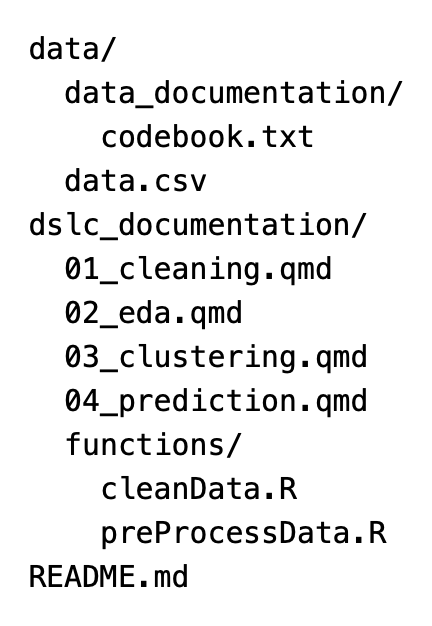
\includegraphics[width=0.275\textwidth,height=\textheight]{chapters/eda/../../figures/project_structure.png}

Le due cartelle principali sono:

\begin{itemize}
\tightlist
\item
  \texttt{data/}: contiene il dataset grezzo (ad esempio,
  \texttt{data.csv}) e una sottocartella con documentazione relativa ai
  dati, come metadati e codebook.
\item
  \texttt{dslc\_documentation/}: raccoglie i file di documentazione e
  codice necessari per le varie fasi del progetto. Questi possono essere
  file .qmd (per Quarto, in R) o .ipynb (per Jupyter Notebook, in
  Python), utilizzati per condurre ed esplorare le analisi. I file sono
  prefissati da un numero per mantenerli in ordine cronologico.
  All'interno di questa cartella, è presente una sottocartella
  \texttt{functions/}, che contiene script .R (per R) o .py (per Python)
  con funzioni utili per le diverse analisi.
\end{itemize}

Un file \texttt{README.md} descrive la struttura del progetto e riassume
il contenuto di ogni file.

Un'organizzazione come quella proposta da Yu \& Barter
(\citeproc{ref-yu2024veridical}{2024}) offre un notevole vantaggio:
permette di specificare i percorsi dei file in modo relativo,
utilizzando come radice la cartella del progetto. Questo rende il
progetto facilmente trasferibile e condivisibile tra diversi utenti o
computer.

\begin{example}[]\protect\hypertarget{exm-}{}\label{exm-}

Per esplorare come gestire l'archiviazione dei dati sul computer e
importarli in Python, consideriamo i dati raccolti da Zetsche et al.
(\citeproc{ref-zetsche_2019future}{2019}) in uno studio che ha esaminato
le aspettative negative come meccanismo chiave nel mantenimento della
depressione. In questo studio, i ricercatori hanno confrontato 30
soggetti con episodi depressivi a un gruppo di controllo di 37 individui
sani, utilizzando il Beck Depression Inventory (BDI-II) per valutare i
livelli di depressione.

Il file CSV contenente questi dati, così come tutti gli altri file
utilizzati in questa dispensa, è memorizzato nella cartella
\texttt{data}, situata all'interno della cartella \texttt{psicometria},
che rappresenta la directory principale del progetto.

Con le istruzioni seguenti, viene specificato il percorso della
directory principale del progetto in relazione alla mia directory
personale:

\begin{Shaded}
\begin{Highlighting}[]
\NormalTok{here}\SpecialCharTok{::}\FunctionTok{here}\NormalTok{()}
\CommentTok{\#\textgreater{} [1] "/Users/corradocaudek/\_repositories/psicometria{-}r"}
\end{Highlighting}
\end{Shaded}

Dopo aver definito \texttt{project\_directory} come directory
principale, è possibile indicare il percorso del file CSV contenente i
dati in modo relativo a \texttt{project\_directory}.

La seguente istruzione permette di importare i dati dal file
\texttt{data.mood.csv} in un DataFrame di pandas.

\begin{Shaded}
\begin{Highlighting}[]
\NormalTok{df }\OtherTok{\textless{}{-}}\NormalTok{ rio}\SpecialCharTok{::}\FunctionTok{import}\NormalTok{(}
\NormalTok{  here}\SpecialCharTok{::}\FunctionTok{here}\NormalTok{(}\StringTok{"data"}\NormalTok{, }\StringTok{"data.mood.csv"}\NormalTok{)}
\NormalTok{)}
\end{Highlighting}
\end{Shaded}

Per conoscere le dimensioni del DataFrame utilizziamo l'istruzione
\texttt{dim()}:

\begin{Shaded}
\begin{Highlighting}[]
\FunctionTok{dim}\NormalTok{(df)}
\CommentTok{\#\textgreater{} [1] 1188   44}
\end{Highlighting}
\end{Shaded}

Il DataFrame ha 1188 righe e 44 colonne. Visualizziamo il nome delle
colonne con il metodo \texttt{.columns}.

\begin{Shaded}
\begin{Highlighting}[]
\NormalTok{df }\SpecialCharTok{|\textgreater{}} \FunctionTok{names}\NormalTok{()}
\CommentTok{\#\textgreater{}  [1] "V1"                  "vpn\_nr"              "esm\_id"             }
\CommentTok{\#\textgreater{}  [4] "group"               "bildung"             "bdi"                }
\CommentTok{\#\textgreater{}  [7] "nr\_of\_episodes"      "nobs\_mood"           "trigger\_counter"    }
\CommentTok{\#\textgreater{} [10] "form"                "traurig\_re"          "niedergeschlagen\_re"}
\CommentTok{\#\textgreater{} [13] "unsicher\_re"         "nervos\_re"           "glucklich\_re"       }
\CommentTok{\#\textgreater{} [16] "frohlich\_re"         "mood\_sad.5"          "mood\_fearful.5"     }
\CommentTok{\#\textgreater{} [19] "mood\_neg.5"          "mood\_happy.5"        "cesd\_sum"           }
\CommentTok{\#\textgreater{} [22] "rrs\_sum"             "rrs\_brood"           "rrs\_reflect"        }
\CommentTok{\#\textgreater{} [25] "forecast\_sad"        "forecast\_fear"       "forecast\_neg"       }
\CommentTok{\#\textgreater{} [28] "forecast\_happy"      "recall\_sad"          "recall\_fear"        }
\CommentTok{\#\textgreater{} [31] "recall\_neg"          "recall\_happy"        "diff\_neg.fore.5"    }
\CommentTok{\#\textgreater{} [34] "diff\_sad.fore.5"     "diff\_fear.fore.5"    "diff\_happy.fore.5"  }
\CommentTok{\#\textgreater{} [37] "diff\_neg.retro.5"    "diff\_sad.retro.5"    "diff\_fear.retro.5"  }
\CommentTok{\#\textgreater{} [40] "diff\_happy.retro.5"  "mood\_sad5\_tm1"       "mood\_neg5\_tm1"      }
\CommentTok{\#\textgreater{} [43] "mood\_fearful5\_tm1"   "mood\_happy5\_tm1"}
\end{Highlighting}
\end{Shaded}

Dato che il DataFrame è troppo grande (1188 righe e 44 colonne),
stampiamo sullo schermo solo le prime 5 righe.

\begin{Shaded}
\begin{Highlighting}[]
\NormalTok{df }\SpecialCharTok{|\textgreater{}} \FunctionTok{head}\NormalTok{()}
\CommentTok{\#\textgreater{}   V1 vpn\_nr esm\_id group bildung bdi nr\_of\_episodes nobs\_mood}
\CommentTok{\#\textgreater{} 1  1    101     10   mdd  abitur  25              2        14}
\CommentTok{\#\textgreater{} 2  2    101     10   mdd  abitur  25              2        14}
\CommentTok{\#\textgreater{} 3  3    101     10   mdd  abitur  25              2        14}
\CommentTok{\#\textgreater{} 4  4    101     10   mdd  abitur  25              2        14}
\CommentTok{\#\textgreater{} 5  5    101     10   mdd  abitur  25              2        14}
\CommentTok{\#\textgreater{} 6  6    101     10   mdd  abitur  25              2        14}
\CommentTok{\#\textgreater{}   trigger\_counter        form traurig\_re niedergeschlagen\_re unsicher\_re}
\CommentTok{\#\textgreater{} 1               5 Forecasting       3.67                3.00        2.33}
\CommentTok{\#\textgreater{} 2               6 Forecasting       3.67                3.67        3.67}
\CommentTok{\#\textgreater{} 3               7 Forecasting       1.67                1.67        2.33}
\CommentTok{\#\textgreater{} 4               8 Forecasting       3.00                3.00        3.00}
\CommentTok{\#\textgreater{} 5              10 Forecasting       3.00                3.00        2.33}
\CommentTok{\#\textgreater{} 6              11 Forecasting       2.33                2.33        2.33}
\CommentTok{\#\textgreater{}   nervos\_re glucklich\_re frohlich\_re mood\_sad.5 mood\_fearful.5 mood\_neg.5}
\CommentTok{\#\textgreater{} 1      3.00         3.00        3.00       3.33           2.67       3.00}
\CommentTok{\#\textgreater{} 2      3.67         2.33        2.33       3.67           3.67       3.67}
\CommentTok{\#\textgreater{} 3      2.33         2.33        3.00       1.67           2.33       2.00}
\CommentTok{\#\textgreater{} 4      3.67         2.33        3.00       3.00           3.33       3.17}
\CommentTok{\#\textgreater{} 5      3.00         3.00        3.00       3.00           2.67       2.83}
\CommentTok{\#\textgreater{} 6      2.33         2.33        3.00       2.33           2.33       2.33}
\CommentTok{\#\textgreater{}   mood\_happy.5 cesd\_sum rrs\_sum rrs\_brood rrs\_reflect forecast\_sad}
\CommentTok{\#\textgreater{} 1         3.00       25      59        14          11            2}
\CommentTok{\#\textgreater{} 2         2.33       25      59        14          11            2}
\CommentTok{\#\textgreater{} 3         2.67       25      59        14          11            2}
\CommentTok{\#\textgreater{} 4         2.67       25      59        14          11            2}
\CommentTok{\#\textgreater{} 5         3.00       25      59        14          11            2}
\CommentTok{\#\textgreater{} 6         2.67       25      59        14          11            2}
\CommentTok{\#\textgreater{}   forecast\_fear forecast\_neg forecast\_happy recall\_sad recall\_fear}
\CommentTok{\#\textgreater{} 1             3          2.5              2        3.5           3}
\CommentTok{\#\textgreater{} 2             3          2.5              2        3.5           3}
\CommentTok{\#\textgreater{} 3             3          2.5              2        3.5           3}
\CommentTok{\#\textgreater{} 4             3          2.5              2        3.5           3}
\CommentTok{\#\textgreater{} 5             3          2.5              2        3.5           3}
\CommentTok{\#\textgreater{} 6             3          2.5              2        3.5           3}
\CommentTok{\#\textgreater{}   recall\_neg recall\_happy diff\_neg.fore.5 diff\_sad.fore.5 diff\_fear.fore.5}
\CommentTok{\#\textgreater{} 1       3.25            2          {-}0.500          {-}1.333            0.333}
\CommentTok{\#\textgreater{} 2       3.25            2          {-}1.167          {-}1.667           {-}0.667}
\CommentTok{\#\textgreater{} 3       3.25            2           0.500           0.333            0.667}
\CommentTok{\#\textgreater{} 4       3.25            2          {-}0.667          {-}1.000           {-}0.333}
\CommentTok{\#\textgreater{} 5       3.25            2          {-}0.333          {-}1.000            0.333}
\CommentTok{\#\textgreater{} 6       3.25            2           0.167          {-}0.333            0.667}
\CommentTok{\#\textgreater{}   diff\_happy.fore.5 diff\_neg.retro.5 diff\_sad.retro.5 diff\_fear.retro.5}
\CommentTok{\#\textgreater{} 1            {-}1.000           0.2500            0.167             0.333}
\CommentTok{\#\textgreater{} 2            {-}0.333          {-}0.4167           {-}0.167            {-}0.667}
\CommentTok{\#\textgreater{} 3            {-}0.667           1.2500            1.833             0.667}
\CommentTok{\#\textgreater{} 4            {-}0.667           0.0833            0.500            {-}0.333}
\CommentTok{\#\textgreater{} 5            {-}1.000           0.4167            0.500             0.333}
\CommentTok{\#\textgreater{} 6            {-}0.667           0.9167            1.167             0.667}
\CommentTok{\#\textgreater{}   diff\_happy.retro.5 mood\_sad5\_tm1 mood\_neg5\_tm1 mood\_fearful5\_tm1}
\CommentTok{\#\textgreater{} 1             {-}1.000            NA            NA                NA}
\CommentTok{\#\textgreater{} 2             {-}0.333          3.33          3.00              2.67}
\CommentTok{\#\textgreater{} 3             {-}0.667          3.67          3.67              3.67}
\CommentTok{\#\textgreater{} 4             {-}0.667          1.67          2.00              2.33}
\CommentTok{\#\textgreater{} 5             {-}1.000          3.00          3.17              3.33}
\CommentTok{\#\textgreater{} 6             {-}0.667          3.00          2.83              2.67}
\CommentTok{\#\textgreater{}   mood\_happy5\_tm1}
\CommentTok{\#\textgreater{} 1              NA}
\CommentTok{\#\textgreater{} 2            3.00}
\CommentTok{\#\textgreater{} 3            2.33}
\CommentTok{\#\textgreater{} 4            2.67}
\CommentTok{\#\textgreater{} 5            2.67}
\CommentTok{\#\textgreater{} 6            3.00}
\end{Highlighting}
\end{Shaded}

\end{example}

\section{Riflessioni Conclusive}\label{riflessioni-conclusive-2}

La bellezza del codice risiede nella sua riusabilità: una volta scritto,
può essere utilizzato tutte le volte che si desidera. Se configurato
correttamente, lo stesso codice applicato agli stessi dati produrrà
sempre gli stessi risultati. Questo principio, noto come
\emph{riproducibilità computazionale}, offre numerosi vantaggi.

\begin{itemize}
\tightlist
\item
  \textbf{Tracciare le modifiche al progetto}: La riproducibilità
  semplifica il monitoraggio delle evoluzioni e dei cambiamenti nel
  progetto, permettendo di vedere come si sviluppa nel tempo.
\item
  \textbf{Riprodurre il proprio lavoro}: L'utente più interessato alla
  riproducibilità sei tu stesso. La capacità di replicare i risultati è
  una caratteristica essenziale, poiché in futuro potresti aver bisogno
  di riprendere in mano il lavoro e comprenderne i dettagli. La
  riproducibilità rende questo processo molto più semplice.
\item
  \textbf{Costruire su basi solide}: Anche altri ricercatori possono
  utilizzare il tuo lavoro come punto di partenza, espandendo e
  approfondendo le conoscenze che hai contribuito a sviluppare.
\end{itemize}

Tuttavia, rendere il codice riproducibile è più difficile di quanto
sembri. In questo capitolo abbiamo esplorato alcuni metodi che possono
aiutare a raggiungere questo obiettivo.

\begin{tcolorbox}[enhanced jigsaw, leftrule=.75mm, title=\textcolor{quarto-callout-note-color}{\faInfo}\hspace{0.5em}{Nota}, colframe=quarto-callout-note-color-frame, colbacktitle=quarto-callout-note-color!10!white, arc=.35mm, toptitle=1mm, breakable, rightrule=.15mm, opacityback=0, bottomrule=.15mm, toprule=.15mm, bottomtitle=1mm, coltitle=black, titlerule=0mm, left=2mm, opacitybacktitle=0.6, colback=white]

Uno dei problemi più importanti nella psicologia contemporanea è la
\emph{crisi di replicabilità}: molti risultati di ricerca non sono
replicabili (\citeproc{ref-open2015estimating}{Collaboration, 2015}). La
\emph{riproducibilità computazionale} si concentra su un obiettivo più
ristretto: ottenere gli stessi risultati utilizzando lo stesso codice
sugli stessi dati.

\end{tcolorbox}

\section{Informazioni sull'Ambiente di
Sviluppo}\label{informazioni-sullambiente-di-sviluppo}

\begin{Shaded}
\begin{Highlighting}[]
\FunctionTok{sessionInfo}\NormalTok{()}
\CommentTok{\#\textgreater{} R version 4.4.2 (2024{-}10{-}31)}
\CommentTok{\#\textgreater{} Platform: aarch64{-}apple{-}darwin20}
\CommentTok{\#\textgreater{} Running under: macOS Sequoia 15.1.1}
\CommentTok{\#\textgreater{} }
\CommentTok{\#\textgreater{} Matrix products: default}
\CommentTok{\#\textgreater{} BLAS:   /Library/Frameworks/R.framework/Versions/4.4{-}arm64/Resources/lib/libRblas.0.dylib }
\CommentTok{\#\textgreater{} LAPACK: /Library/Frameworks/R.framework/Versions/4.4{-}arm64/Resources/lib/libRlapack.dylib;  LAPACK version 3.12.0}
\CommentTok{\#\textgreater{} }
\CommentTok{\#\textgreater{} locale:}
\CommentTok{\#\textgreater{} [1] C/UTF{-}8/C/C/C/C}
\CommentTok{\#\textgreater{} }
\CommentTok{\#\textgreater{} time zone: Europe/Rome}
\CommentTok{\#\textgreater{} tzcode source: internal}
\CommentTok{\#\textgreater{} }
\CommentTok{\#\textgreater{} attached base packages:}
\CommentTok{\#\textgreater{} [1] stats4    stats     graphics  grDevices utils     datasets  methods  }
\CommentTok{\#\textgreater{} [8] base     }
\CommentTok{\#\textgreater{} }
\CommentTok{\#\textgreater{} other attached packages:}
\CommentTok{\#\textgreater{}  [1] mokken\_3.1.2         poLCA\_1.6.0.1        scatterplot3d\_0.3{-}44}
\CommentTok{\#\textgreater{}  [4] mirt\_1.43            lattice\_0.22{-}6       MASS\_7.3{-}61         }
\CommentTok{\#\textgreater{}  [7] viridis\_0.6.5        viridisLite\_0.4.2    ggpubr\_0.6.0        }
\CommentTok{\#\textgreater{} [10] ggExtra\_0.10.1       gridExtra\_2.3        patchwork\_1.3.0     }
\CommentTok{\#\textgreater{} [13] bayesplot\_1.11.1     psych\_2.4.6.26       scales\_1.3.0        }
\CommentTok{\#\textgreater{} [16] markdown\_1.13        knitr\_1.49           lubridate\_1.9.3     }
\CommentTok{\#\textgreater{} [19] forcats\_1.0.0        stringr\_1.5.1        dplyr\_1.1.4         }
\CommentTok{\#\textgreater{} [22] purrr\_1.0.2          readr\_2.1.5          tidyr\_1.3.1         }
\CommentTok{\#\textgreater{} [25] tibble\_3.2.1         ggplot2\_3.5.1        tidyverse\_2.0.0     }
\CommentTok{\#\textgreater{} [28] here\_1.0.1          }
\CommentTok{\#\textgreater{} }
\CommentTok{\#\textgreater{} loaded via a namespace (and not attached):}
\CommentTok{\#\textgreater{}  [1] mnormt\_2.1.1         pbapply\_1.7{-}2        testthat\_3.2.1.1    }
\CommentTok{\#\textgreater{}  [4] permute\_0.9{-}7        airports\_0.1.0       rlang\_1.1.4         }
\CommentTok{\#\textgreater{}  [7] magrittr\_2.0.3       rio\_1.2.3            compiler\_4.4.2      }
\CommentTok{\#\textgreater{} [10] mgcv\_1.9{-}1           vctrs\_0.6.5          pkgconfig\_2.0.3     }
\CommentTok{\#\textgreater{} [13] fastmap\_1.2.0        backports\_1.5.0      utf8\_1.2.4          }
\CommentTok{\#\textgreater{} [16] promises\_1.3.0       rmarkdown\_2.29       sessioninfo\_1.2.2   }
\CommentTok{\#\textgreater{} [19] tzdb\_0.4.0           openintro\_2.5.0      xfun\_0.49           }
\CommentTok{\#\textgreater{} [22] jsonlite\_1.8.9       later\_1.3.2          styler\_1.10.3       }
\CommentTok{\#\textgreater{} [25] Deriv\_4.1.6          broom\_1.0.7          parallel\_4.4.2      }
\CommentTok{\#\textgreater{} [28] cluster\_2.1.6        R6\_2.5.1             stringi\_1.8.4       }
\CommentTok{\#\textgreater{} [31] parallelly\_1.39.0    car\_3.1{-}3            brio\_1.1.5          }
\CommentTok{\#\textgreater{} [34] Rcpp\_1.0.13{-}1        future.apply\_1.11.3  snow\_0.4{-}4          }
\CommentTok{\#\textgreater{} [37] audio\_0.1{-}11         cherryblossom\_0.1.0  pacman\_0.5.1        }
\CommentTok{\#\textgreater{} [40] R.utils\_2.12.3       R.cache\_0.16.0       httpuv\_1.6.15       }
\CommentTok{\#\textgreater{} [43] Matrix\_1.7{-}1         splines\_4.4.2        timechange\_0.3.0    }
\CommentTok{\#\textgreater{} [46] tidyselect\_1.2.1     abind\_1.4{-}8          vegan\_2.6{-}8         }
\CommentTok{\#\textgreater{} [49] codetools\_0.2{-}20     miniUI\_0.1.1.1       dcurver\_0.9.2       }
\CommentTok{\#\textgreater{} [52] curl\_6.0.1           listenv\_0.9.1        shiny\_1.9.1         }
\CommentTok{\#\textgreater{} [55] withr\_3.0.2          evaluate\_1.0.1       future\_1.34.0       }
\CommentTok{\#\textgreater{} [58] pillar\_1.9.0         carData\_3.0{-}5        generics\_0.1.3      }
\CommentTok{\#\textgreater{} [61] rprojroot\_2.0.4      hms\_1.1.3            munsell\_0.5.1       }
\CommentTok{\#\textgreater{} [64] globals\_0.16.3       xtable\_1.8{-}4         glue\_1.8.0          }
\CommentTok{\#\textgreater{} [67] RPushbullet\_0.3.4    tools\_4.4.2          data.table\_1.16.2   }
\CommentTok{\#\textgreater{} [70] beepr\_2.0            SimDesign\_2.17.1     ggsignif\_0.6.4      }
\CommentTok{\#\textgreater{} [73] grid\_4.4.2           colorspace\_2.1{-}1     nlme\_3.1{-}166        }
\CommentTok{\#\textgreater{} [76] Formula\_1.2{-}5        usdata\_0.3.1         cli\_3.6.3           }
\CommentTok{\#\textgreater{} [79] fansi\_1.0.6          gtable\_0.3.6         R.methodsS3\_1.8.2   }
\CommentTok{\#\textgreater{} [82] rstatix\_0.7.2        digest\_0.6.37        progressr\_0.15.1    }
\CommentTok{\#\textgreater{} [85] GPArotation\_2024.3{-}1 farver\_2.1.2         htmltools\_0.5.8.1   }
\CommentTok{\#\textgreater{} [88] R.oo\_1.27.0          lifecycle\_1.0.4      mime\_0.12}
\end{Highlighting}
\end{Shaded}

\section*{Bibliografia}\label{bibliografia-4}
\addcontentsline{toc}{section}{Bibliografia}

\markright{Bibliografia}

\phantomsection\label{refs}
\begin{CSLReferences}{1}{0}
\bibitem[\citeproctext]{ref-angrist2010credibility}
Angrist, J. D., \& Pischke, J.-S. (2010). The credibility revolution in
empirical economics: How better research design is taking the con out of
econometrics. \emph{Journal of economic perspectives}, \emph{24}(2),
3--30.

\bibitem[\citeproctext]{ref-baker20161}
Baker, M. (2016). 1,500 scientists lift the lid on reproducibility.
\emph{Nature}, \emph{533}(7604).

\bibitem[\citeproctext]{ref-bishop2019psychology}
Bishop, D. (2019). \emph{The psychology of experimental psychologists:
Overcoming cognitive constraints to improve research}.

\bibitem[\citeproctext]{ref-button2013power}
Button, K. S., Ioannidis, J. P., Mokrysz, C., Nosek, B. A., Flint, J.,
Robinson, E. S., \& Munafò, M. R. (2013). Power failure: why small
sample size undermines the reliability of neuroscience. \emph{Nature
Reviews Neuroscience}, \emph{14}(5), 365--376.

\bibitem[\citeproctext]{ref-open2015estimating}
Collaboration, O. S. (2015). Estimating the reproducibility of
psychological science. \emph{Science}, \emph{349}(6251), aac4716.

\bibitem[\citeproctext]{ref-eronen2021theory}
Eronen, M. I., \& Bringmann, L. F. (2021). The theory crisis in
psychology: How to move forward. \emph{Perspectives on Psychological
Science}, \emph{16}(4), 779--788.

\bibitem[\citeproctext]{ref-definetti1970teoria}
Finetti, B. de. (1970). \emph{Teoria delle probabilit{à}: sintesi
introduttiva con appendice critica}. Einaudi.

\bibitem[\citeproctext]{ref-funder2014improving}
Funder, D. C., Levine, J. M., Mackie, D. M., Morf, C. C., Sansone, C.,
Vazire, S., \& West, S. G. (2014). Improving the dependability of
research in personality and social psychology: Recommendations for
research and educational practice. \emph{Personality and Social
Psychology Review}, \emph{18}(1), 3--12.

\bibitem[\citeproctext]{ref-gansch2020system}
Gansch, R., \& Adee, A. (2020). System theoretic view on uncertainties.
\emph{2020 Design, Automation \& Test in Europe Conference \& Exhibition
(DATE)}, 1345--1350.

\bibitem[\citeproctext]{ref-gelman1995bayesian}
Gelman, A., Carlin, J. B., Stern, H. S., \& Rubin, D. B. (1995).
\emph{Bayesian data analysis}. Chapman; Hall/CRC.

\bibitem[\citeproctext]{ref-gelman2020regression}
Gelman, A., Hill, J., \& Vehtari, A. (2020). \emph{Regression and Other
Stories}. Cambridge University Press.

\bibitem[\citeproctext]{ref-gelman2013garden}
Gelman, A., \& Loken, E. (2013). The garden of forking paths: Why
multiple comparisons can be a problem, even when there is no {«fishing
expedition»} or {«p-hacking»} and the research hypothesis was posited
ahead of time. \emph{Department of Statistics, Columbia University},
\emph{348}(1-17), 3.

\bibitem[\citeproctext]{ref-gelman2014statistical}
Gelman, A., \& Loken, E. (2014). The statistical crisis in science.
\emph{American scientist}, \emph{102}(6), 460--465.

\bibitem[\citeproctext]{ref-huntington2021effect}
Huntington-Klein, N. (2021). \emph{The effect: An introduction to
research design and causality}. Chapman; Hall/CRC.

\bibitem[\citeproctext]{ref-ioannidis2005most}
Ioannidis, J. P. (2005). Why most published research findings are false.
\emph{PLoS medicine}, \emph{2}(8), e124.

\bibitem[\citeproctext]{ref-ioannidis2019have}
Ioannidis, J. P. (2019). What have we (not) learnt from millions of
scientific papers with P values? \emph{The American Statistician},
\emph{73}(sup1), 20--25.

\bibitem[\citeproctext]{ref-korbmacher2023replication}
Korbmacher, M., Azevedo, F., Pennington, C. R., Hartmann, H., Pownall,
M., Schmidt, K., Elsherif, M., Breznau, N., Robertson, O., Kalandadze,
T., et al. (2023). The replication crisis has led to positive
structural, procedural, and community changes. \emph{Communications
Psychology}, \emph{1}(1), 3.

\bibitem[\citeproctext]{ref-labatut2021abbiamo}
Labatut, B. (2021). \emph{Quando abbiamo smesso di capire il mondo}.
Adelphi Edizioni spa.

\bibitem[\citeproctext]{ref-larson2023bayesian}
Larson, C., Kaplan, D., Girolamo, T., Kover, S. T., \& Eigsti, I.-M.
(2023). A Bayesian statistics tutorial for clinical research: Prior
distributions and meaningful results for small clinical samples.
\emph{Journal of Clinical Psychology}, \emph{79}(11), 2602--2624.

\bibitem[\citeproctext]{ref-lilienfeld2020psychological}
Lilienfeld, S. O., \& Strother, A. N. (2020). Psychological measurement
and the replication crisis: Four sacred cows. \emph{Canadian
Psychology/Psychologie Canadienne}, \emph{61}(4), 281--288.

\bibitem[\citeproctext]{ref-lindley2013understanding}
Lindley, D. V. (2013). \emph{Understanding uncertainty}. John Wiley \&
Sons.

\bibitem[\citeproctext]{ref-maul2016philosophical}
Maul, A., Irribarra, D. T., \& Wilson, M. (2016). On the philosophical
foundations of psychological measurement. \emph{Measurement}, \emph{79},
311--320.

\bibitem[\citeproctext]{ref-McElreath_rethinking}
McElreath, R. (2020). \emph{Statistical rethinking: {A} {Bayesian}
course with examples in {R} and {Stan}} (2nd Edition). CRC Press.

\bibitem[\citeproctext]{ref-meehl1967theory}
Meehl, P. E. (1967). Theory-testing in psychology and physics: A
methodological paradox. \emph{Philosophy of science}, \emph{34}(2),
103--115.

\bibitem[\citeproctext]{ref-munger2023temporal}
Munger, K. (2023). Temporal validity as meta-science. \emph{Research \&
Politics}, \emph{10}(3), 20531680231187271.

\bibitem[\citeproctext]{ref-murray2024measuring}
Murray, E. J., \& Carr, K. C. (2024). Measuring Racial Sentiment Using
Social Media Is Harder Than It Seems. \emph{Epidemiology}, \emph{35}(1),
60--63.

\bibitem[\citeproctext]{ref-nobles2000shades}
Nobles, M. (2000). \emph{Shades of citizenship: Race and the census in
modern politics}. Stanford University Press.

\bibitem[\citeproctext]{ref-oberauer2019addressing}
Oberauer, K., \& Lewandowsky, S. (2019). Addressing the theory crisis in
psychology. \emph{Psychonomic Bulletin \& Review}, \emph{26},
1596--1618.

\bibitem[\citeproctext]{ref-pearl2018book}
Pearl, J., \& Mackenzie, D. (2018). \emph{The book of why: the new
science of cause and effect}. Basic books.

\bibitem[\citeproctext]{ref-shrout2018psychology}
Shrout, P. E., \& Rodgers, J. L. (2018). Psychology, science, and
knowledge construction: Broadening perspectives from the replication
crisis. \emph{Annual Review of Psychology}, \emph{69}(1), 487--510.

\bibitem[\citeproctext]{ref-simmons2011false}
Simmons, J. P., Nelson, L. D., \& Simonsohn, U. (2011). False-positive
psychology: Undisclosed flexibility in data collection and analysis
allows presenting anything as significant. \emph{Psychological science},
\emph{22}(11), 1359--1366.

\bibitem[\citeproctext]{ref-stevens_46}
Stevens, S. S. (1946). On the theory of scales of measurement.
\emph{Science}, \emph{103}(2684), 677--680.

\bibitem[\citeproctext]{ref-tackett2019psychology}
Tackett, J. L., Brandes, C. M., King, K. M., \& Markon, K. E. (2019).
Psychology's replication crisis and clinical psychological science.
\emph{Annual Review of Clinical Psychology}, \emph{15}(1), 579--604.

\bibitem[\citeproctext]{ref-van2024productive}
Van Dongen, N., Bork, R. van, Finnemann, A., Haslbeck, J., Maas, H. L.
van der, Robinaugh, D. J., Ron, J. de, Sprenger, J., \& Borsboom, D.
(2024). Productive explanation: A framework for evaluating explanations
in psychological science. \emph{Psychological Review}.

\bibitem[\citeproctext]{ref-wagenmakers2018bayesian}
Wagenmakers, E.-J., Marsman, M., Jamil, T., Ly, A., Verhagen, J., Love,
J., Selker, R., Gronau, Q. F., Šmı́ra, M., Epskamp, S., et al. (2018).
Bayesian inference for psychology. Part I: Theoretical advantages and
practical ramifications. \emph{Psychonomic Bulletin \& Review},
\emph{25}, 35--57.

\bibitem[\citeproctext]{ref-yarkoni2022generalizability}
Yarkoni, T. (2022). The generalizability crisis. \emph{Behavioral and
Brain Sciences}, \emph{45}, e1.

\bibitem[\citeproctext]{ref-yu2024veridical}
Yu, B., \& Barter, R. L. (2024). \emph{Veridical data science: The
practice of responsible data analysis and decision making}. MIT Press.

\bibitem[\citeproctext]{ref-zetsche_2019future}
Zetsche, U., Buerkner, P.-C., \& Renneberg, B. (2019). Future
expectations in clinical depression: biased or realistic? \emph{Journal
of Abnormal Psychology}, \emph{128}(7), 678.

\end{CSLReferences}




\end{document}
